\documentclass[letterpaper,conference]{IEEEtran}

%Paquete para citar
\usepackage{natbib}
% Primero apretar f11, despues f6 y luego f7
%Para referenciar una cita entera, poner \citep{}
% Para referenciar una cita dentro de un mismo texto, colocar \citet{} 
\usepackage{url}
%Paquete para gráficos, por ejemplo colocar imágenes
\usepackage[pdftex]{graphicx}

%Paquete para ecuacioens y/o otros elementos matemáticos
\usepackage{amsmath,amsfonts,amssymb,amsthm, bm}
\usepackage{mathtools}
\usepackage[table,xcdraw]{xcolor}
\DeclarePairedDelimiter\ceil{\lceil}{\rceil}
\DeclarePairedDelimiter\floor{\lfloor}{\rfloor}

%Paquetes para alinear texto y/o ecuaciones
\usepackage{array}

% Distintas opciones de itemizdo
\usepackage{enumitem}

%Opciones de tabla
\usepackage{multirow}



\begin{document}

\title{Modelo de asignación de vehículos de recolección de escombros en desastres naturales}

\author{\IEEEauthorblockN{Samantha Reid Calderón}
\IEEEauthorblockA{MSc., Docente\\ Departamento de Ciencias de la Ingeniería\\
Universidad Andrés Bello \\
Santiago, Chile\\
Email:s.reid.cal@gmail.com}
\and
\IEEEauthorblockN{Isaac Montero Jara}
\IEEEauthorblockA{Estudiante de Ingeniería \\ Facultad de Ingeniería\\ Universidad Andrés Bello \\
Santiago, Chile\\
Email: i.monterojara@uandresbello.edu}}

% Para colocar el título
\maketitle

%Para ponerle número de página al documento
\thispagestyle{plain}
\pagestyle{plain}

\begin{abstract}
Se aborda el problema de recolección de escombros de edificios posterior de un desastre natural. Se presenta un modelo de programación de tareas que entrega la planificación de de los equipos de limpieza de escombros, maximizando el número de edificios limpiados, tales como los hospitales y colegios. El caso de estudio se presenta en la ciudad de Iquique, Chile. Los resultados se presenta el desarrollo del modelo propuesto, integrando un factor de preferencía en la limpieza de edificios hacia los primeros días del horizonte de planificación, posteriormente se realizan variaciones del modelamiento para verificar su comportamiento\\ 
%%%%%%%%%%%%%%%%%%%%%%%%%%%%%%%%%%%%%%%%%%%%%%%%%%%%%%% VERIFICAR...
\end{abstract}
\begin{IEEEkeywords}
Recolección de escombros, Logística humanitaria, Fase de recuperación, Ruteo vehicular.
\end{IEEEkeywords}

\IEEEpeerreviewmaketitle

\section{INTRODUCCIÓN}

Los desastres naturales se definen como “las interrupciones que afectan físicamente a un sistema en su conjunto y amenaza sus prioridades y objetivos” \citep{van2006humanitarian}. Se han registrado 3.155 eventos naturales a nivel mundial, produciendo pérdidas humanas, infraestructura y económicas \citep{emdat}.

Estos presentan un ciclo de vida de cuatro etapas: mitigación, preparación, respuesta y preparación. En las primeras dos etapas se ven todas las actividades relacionadas a la preparación ante un desastre (localización de alarmas o albergues, entre otros). En la fase de respuesta se ven las actividades relacionadas con las primeras 72 horas producido una eventualidad, tales como distribución de suministros o recolección de víctimas. En la última fase se organizan actividades de apoyo para devolver la infraestructura e actividades rutinarias a una comunidad \citep{Feng2003}. Esta fase comienza cuando la emergencia se ha estabilizado y ya no existe un peligro latente para la población, finalizando con la recuperación total de la comunidad \citep{lindell2006wiley}. Se realizan actividaddes de corto y largo plazo para eliminar todo rastro físico, dándole importancia al reciclaje, almacenamiento y reducción de desechos. Una de estas actividades es la recolección de escombros para mantener las vías de acceso a hospitales, albergues y otros edificios importantes.

Se propone un modelo lineal de asignación de vehículos en un horizonte de tiempo determinado, maximizando la cantidad de edificios limpiados. El caso de estudio tiene lugar en la ciudad de Iquique, Chile, debido a la alta cantidad de desastres registrados en la zona \citep{sismologia}.

La metodología considera priorizar los edificios según su importancia para la comunidad, contemplando una flota heterogénea de vehículos recolectores. Con ello se diseña un modelo lineal programado en AMPL Gurobi, con tiempos de cómputo de 18,000 segundos. En los resultados se muestra el comportamiento del modelo, integrando un factor de prioridad de limpieza hacia los primeros días del horizonte de planificación.

%%%%%%%%%%%%%%%%%%%%%%%%%%%%%%%%%%%%%%%%%

El resto del documento se organiza de la siguiente manera. En la sección 2 se presenta la revisión de la literatura, donde se dan a conocer trabajos similares. En la sección 3 se presenta la metodología. En la sección 4 se presenta el caso de estudio con los datos utilizados. En la sección 5 se presentan los resultados y sus análisis. Finalmente, en la sección 6 se presentan las conclusiones del trabajo y sus futuras investigaciones.

\section{REVISIÓN DE LA LITERATURA}

Tras ocurrido un desastre, es importante recuperar la vida previa a la comunidad. Uno de los elementos a considerar son las políticas de reconstrucción y restauración de las redes \citet{Feng2003}. Por lo tanto, se deben encontrar soluciones que permitan optimizar el uso de los recursos destinados a actividades de limpieza y recolección.

Existen autores que abordan el problema a través de ruteo vehicular. \citet{Karlaftis2007} proponen un modelo de tres etapas, donde maximiza la importancia de los nodos, asigna recursos y minimiza costos de reparación, enfocado en puentes. \citet{Liberatore2014} minimizan el tiempo necesario para las reparaciones de emergencia y distribución de artículos de ayuda a través de un modelo multicriterio, donde incorpora el tiempo, costo, confiabilidad, seguridad y satisfacción de la demanda. \citet{Aksu2014} maximiza la accesibilidad a la red para evacuar a los sobrevivientes y remover desechos de las rutas. \citet{MayaDuque2016} realizan una planificación de equipos de limpieza y su ruteo dentro de la red para limpiar edificios. Por último, \citet{Kasaei2016} desarrollan un modelo lineal que limpia caminos bloqueados, minimizando el tiempo de reconexión de la red y maximizando el beneficio total de reconexión dentro de un tiempo dado.

De manera similar, existen estudios que abordan el problema a través de planificación y asignación. \citet{Feng2003} proponen un modelo multiobjetivo de limpieza de edificios, donde maximiza el largo de las rutas accesibles, el total de vidas salvadas y minimiza el riesgo. \citet{Brooks2013} determinan la estrategia para asignar los vehículos entre los sitios de recogida y almacenamiento temporal de escombros, maximizando el flujo de la red. \citet{Ransikarbum2016} desarrollan un modelo para decisiones estratégicas en la distribución de suministros y restauración de la red, maximizando equidad, minimizando demanda insatisfecha y costos. \citet{Akbari2017} generan una planificación para equipos de limpieza para reconectar la red.

Además, en los últimos años se ha incorporado el factor de reciclaje en esta fase. \citet{Boonmee2018} realizan un modelo de localización y asignación de centros de reciclaje, minimizado los costos y penalizando daños al ambiente. \citet{Wang2019} proponen un modelo de asignación multiobjetivo que minimiza costos de remoción de escombros, tiempo total de procesamiento y maximiza el reciclaje.

El modelo presentado tiene como objetivo maximizar la preferencia de limpieza de los edificios hacia los primeros días de trabajo, brindando prioridad a los edificios a limpiar por día, agregando un ponderador de prioridad hacia los primeros días de jornada laboral, declarando como edificios a hospitales y colegios de la ciudad a estudiar.

El resumen, ésta tesis contribuye a la literatura en la remoción de escombros en: (a) agregar un ponderador al modelo, el cual beneficia a la limpieza de cada edificio hacia los primeros días de jornada laboral, asumiendo que durante el transcurso del tiempo las zonas con mayor prioridad serán limpiadas; (b) se efectúa el modelo con datos reales de la zona y simulaciones del software HAZUS.

\section{METODOLOGÍA}

\subsection{Descripción del problema}

Se cuenta con un grafo $G(N,A)$, donde $N$ son los nodos de la red y $A$ los arcos. Además, el conjunto de nodo está conformado por un conjunto de edificios $E$ y un depósito $O$. Por otro lado, se cuenta con una flota homogénea de $K$ vehículos que prestan un servicio de recolección de escombros, los cuales realizan $V$ vueltas dentro de $D$ días en un horizonte de planificación.

Cada edificio cuenta con un ponderador de preferencia $\alpha_e$, el cual es mayor según la importancia que otorga este edificio a la comunidad dentro de un desastre; cantidad $C_e$ de escombros que deben ser recolectados; y un tiempo de trabajo de carga de retiro de escombros $theta_e$. Con respecto a los camiones, estos cuentan con una capacidad $q$ para recolectar escombros.

Además, se cuenta con un ponderador $\beta^d$, cuyo valor disminuye a medida que avanzan los días; y con un tiempo de máximo de trabajo $T_{MAX}$ para cada camión.

\subsection{Supuestos}

\begin{enumerate}[label=\roman*.]
	\item La red vial, distancias, tiempos de operación y cantidad de escombros son datos previamente conocidos.
	\item Se establece previamente una jornada laboral limitada.	
	\item Un nodo representa un único edificio.
	\item Todos los vehículos se encuentran disponibles dentro del horizonte de planificación.	
	\item Para cada vuelta, un vehículo debe iniciar y terminar el recorrido en el depósito.
	\item En cada edificio se encuentra operativa una máquina para cargar los escombros al vehículo.	
	\item No se permite el traslado entre edificios.	
	\item No se considera el re-abastecimiento de combustible.
	\item No se consideran los tiempos de operación en el depósito.
\end{enumerate}

\subsection{Formulación del Modelo}

\subsection{Conjuntos}
Se consideraron los siguientes conjuntos:
\begin{itemize}
	\item $N$: Conjunto de nodos.
	\item $E \subseteq N$: Conjunto de edificios.
	\item $O \subseteq N$: Conjunto de depósitos.
	\item $A = \{o,i\} \cup \{i,o\} / i \in E, o \in O$: Conjunto de arcos.
	\item $K$: Conjunto de camiones.
	\item $V$: Conjunto de vueltas.
	\item $D$: Conjunto de días.
\end{itemize}

\subsection{Parámetros}
Los parámetros considerados son los siguientes:

\begin{itemize}
	\item $\alpha_e$: Escalar de preferencia del edificio $e \in E$.
	\item $\beta^{d}$: Ponderador de día $d \in D$.
	\[ \beta^d = \dfrac{|D|-(d-1)}{|D|} \]
	\item $q$: Capacidad del vehículo. 
	\item $c_e$: Cantidad de escombros de cada edificio $e \in E$.
	\item $\gamma_{ij}$: Tiempo de desplazamiento de nodo $(i,j) \in A$.
	\item $\theta_{e}$: Tiempo de trabajo de retiro de escombros del edificio $e \in E$.
	\item $tmax$: Tiempo máximo de trabajo diario para un camión.
	\item $\lambda_e$: Cantidad de vueltas necesarias para limpiar completamente edificio $e \in E$.
%	\[ \lambda_e = \lceil \frac{ c_e }{q} \rceil \]

	\[ \lambda_e = \ceil*{ \frac{ c_e }{q} } \]
	\item $M$: Número muy grande.
\end{itemize}

\subsection{Variables}
Las variables de decisión elaboradas se presentan a continuación.

\begin{itemize}
	\item $x_{ij}^{kvd}$: 1 si se desplaza desde el arco $(i,j) \in A$	con el camión $k \in K$ en la vuelta $v \in V$ y en el día $d \in D$, 0 si no.
	\item $y_{e}^{d}$: 1 si el edificio $e \in E$ se limpia completamente el día $d \in D$, 0 si no.
	\item $w_{e}^{kvd}$: Cantidad de escombros retirados del edificio $e \in E$ por el camión $k \in K$, en la vuelta $v \in V$ y en el día $d \in D$.
	\item $t^{kd}$: Tiempo de trabajo del camión $k \in K$ en el día $d \in D$.
	\item $z_e^d$: Variable que guarda el valor de la función objetivo. % AGREGAR.
\end{itemize}

\subsection{Modelo Matemático}

A continuación, se presenta el modelo matemático:

{\small
\begin{align}
	& \max \quad \sum_{d \in D} \sum_{e \in E} \beta^{d}  \alpha_e z_e^d  \label{eq1}
\end{align}
}

La función (\ref{eq1}) maximiza la preferencia de limpieza de los edificios hacia los primeros días del horizonte de planificación.

{\small
\begin{align}
	& \sum_{k \in K} \sum_{v \in V} \sum_{d \in D} x_{ie}^{kvd} \leq \lambda_e \hspace{1cm} \forall i \in O , e \in E \label{eq2} \\
	& x_{ie}^{kvd} = x_{ei}^{kvd} \hspace{1cm} \forall i \in O, e \in E k \in K, v \in V, d \in D \label{eq3}
\end{align}
}

La restricción (\ref{eq2}) limita que un edificio se puede visitar, a lo más, la cantidad de veces necesarias para limpiarlo completamente. La restricción (\ref{eq3}) indica que el vehículo debe devolverse al depósito cada vez que visita un edificio.

{\small
\begin{align}
 	& \sum_{e \in E} \sum_{v \in V} x_{ei}^{kv(d+1)} \leq \sum_{e \in E} \sum_{v \in V} x_{ei}^{kvd}   \label{eq4} \\ \nonumber
 	& \hspace{2.9cm} \forall i \in O, k \in K, d \in D / (d+1) \in D   \\
	& \sum_{e \in E} x_{ei}^{k(v+1)d} \leq \sum_{e \in E} x_{ei}^{kvd} \label{eq5} \\ \nonumber
	& \hspace{2cm} \forall i \in O, k \in K, v \in V, d \in D /(v+1) \in V 
\end{align}
}

La restricción (\ref{eq4}) establece la secuencia de días, mientras que (\ref{eq5}) establece la secuencia de vueltas.

{\small
\begin{align}
	& \sum_{e \in E} w_{e}^{kvd} \leq q & \forall k \in K, v \in V, d \in D \label{eq6} \\
	& \sum_{k \in K} \sum_{v \in V} \sum_{d \in D} w_{e}^{kvd} \leq c_e & \forall e \in E \label{eq7}
\end{align}
}

La restricción (\ref{eq6}) establece que la carga retirada de un edificio no puede sobrepasar la capacidad del camión, mientras que (\ref{eq7}) establece que no se puede retirar más que la disponibilidad de escombros que presente el edificio.

{\small
\begin{align}
	& t^{kd} = \sum_{(i,j) \in A} \sum_{v \in V} \gamma_{ij} x_{ij}^{kvd} + \sum_{e \in E} \sum_{v \in V} \theta_{e} {w_{e}^{kvd}}{q} \label{eq8} \\ \nonumber
	& \hspace{5.65cm} \forall k \in K, d \in D \\
	& t^{kd} \leq T_{MAX} \hspace{4.1cm} k \in K, d \in D \label{eq9} \\
	& y_{e}^{d} \leq \sum_{k \in K} \sum_{v \in V} \frac{w_{e}^{kvd}}{c_e} \hspace{3cm} \forall e \in E, d \in D \label{eq10}
\end{align}
}

La restricción (\ref{eq8}) calcula el tiempo de trabajo diario de un vehículo. La restricción (\ref{eq9}) limita la jornada laboral diaria. La restricción (\ref{eq10}) identifica el día que se termina de limpiar cada edificio.

{\small
\begin{align}
	& w_{e}^{kvd} \leq M x_{e}^{kvd} \hspace{1.55cm} \forall k \in K, e \in E, v \in V, d \in D \label{eq11} \\
	& x_{ij}^{kvd}, y_{e}^{kvd} \in \{0,1 \} \label{eq12} \\ \nonumber
	& \hspace{2.2cm} \forall (i,j) \in A, e \in E, k \in K, v \in V, d \in D \\
	& w_{e}^{kvd}, t^{kd} \geq 0 \label{eq13} \\ \nonumber
	& \hspace{2.7cm} \forall e \in E, k \in K, v \in V, d \in D
\end{align}
}

Las restricciones (\ref{eq11}) relacionan las variables. Las restricciones (\ref{eq12}) y (\ref{eq13}) indican el dominio de las variables.

\section{Caso de Estudio}

\subsection{Área de estudio}

El caso de estudio se realizó en la región de Tarapacá en la ciudad de Iquique, Chile, visualizada en la \ref{fig:fig2}. Esta ciudad cuenta con una población de 191.468 personas y una superficie de 2.262,4 $m^{2}$ \citep{CENSO2017}.

\begin{figure}[h!]
\centering
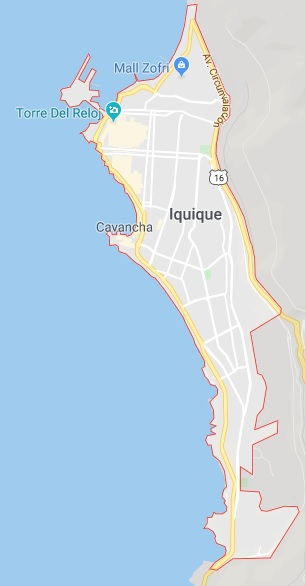
\includegraphics[scale=0.5]{Figuras/iquique1.jpg}
\caption{Mapa de Iquique. Fuente: Google Maps (2019)}
\label{fig:fig2}
\end{figure}

Esta región está propensa a sufrir catástrofes naturales debido a su ubicación sobre la placa Sudamericana la cual produce un movimiento contrario a la placa de Nazca \citep{sismologia}. Según \citet{emdat}, se cuenta con un historial de cuatro sismos de gran magnitud en los últimos 25 años, debido a que superan los 7.0 grados de magnitud. En la Tabla \ref{tab:tab1} se muestran los eventos sísmicos desde 1900, cuyas leyendas son: Magnitud de ondas superficiales (Ms) y Magnitud del momento (Mw) \citep{sismologia}.

\begin{table}[h!]
\resizebox{9cm}{!} {
	\centering
	\begin{tabular}{c|c|c|c|c} \hline
	Fecha	& Latitud &	Longitud & Magnitud  Ms / Mw & Profundidad (km) \\ \hline
	15-09-1911  & -20	& -72 	 & 7.3 (Ms) & - \\ 
	23-02-1933  & -20   & -71	 & 7.6 (Ms) & 40  \\ 
	01-12-1943  & -21	& -69    & 7   (Ms) & 100 \\ 
	25-04-1949	& -19.75& -69	 & 7.3 (Ms) & 110 \\ 
	08-01-1956	& -19   & -70	 & 7.1 (Ms) & 11 \\ 
	13-06-1959	& -20.42& -69 	 & 7.5 (Ms) & 83 \\ 
	29-11-1976 	& -20.52& -68.919& 7.3 (Ms) & 82  \\ 
	08-08-1987	& -19	& -70	 & 7.1 (Ms) & 42  \\ 
	13-06-2005	& -19.895&-69.125& 7.8 (Ms/Mw) & 108 \\ 
	01-04-2014	& -19.572&-70.908& 8.2 (Mw) & 38.9  \\ \hline
	\end{tabular}
	}
	\caption{Historial de terremotos Región de Tarapacá, a partir del año 1900. Fuente: \citep{guc}}.
	\label{tab:tab1} 
\end{table}

\subsection{Recopilación de datos}

\subsubsection{Red vial y obtención de escombros}

La red vial se obtuvo a través del Ministerio de Transporte y Telecomunicaciones de Chile, la cual se compone de 1655 manzanas censales \citet{CENSO2017}. Estos datos fueron procesados en el software ArcGis 10.1, del cual se obtuvo la matriz de distancia entre los nodos de la red.

Por otro lado, la cantidad de escombros para cada una fue obtenida a través del software HAZUS 2.1, a partir de una simulación de un escenario de magnitud 8.0 Mw. Se tomó en consideración sólo los escombros de tipo madera y ladrillos, puesto que los demás requieren de equipamiento más avanzado \citep{hasuz}.

\subsubsection{Edificios}

Durante la fase de recuperación es importante mantener las vías de acceso despejadas a hospitales, colegios y otros edificios de interés. Estos se utilizan como recurso para la comunidad con el fin de albergar personas y/o prestar servicios de primeros auxilios \citet{lindell2006wiley}. En total, se consideraron 16 centros de salud y 65 establecimientos de educación, cuyo detalle se presenta en el Anexo \ref{anexo1} y su distribución espacial en la Figura \ref{fig:fig3}.

\begin{figure}[h!]
	\centering
	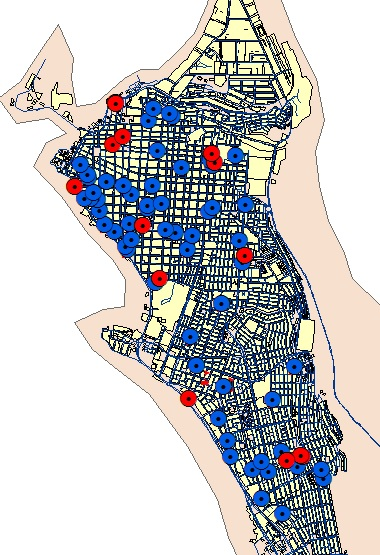
\includegraphics[scale=0.55]{Figuras/mapaarc.JPG}
	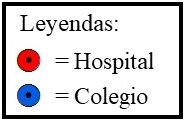
\includegraphics[scale=0.5]{Figuras/simb1.jpg}
	\caption{Centros de Salud y Establecimientos de Educación en Iquique. Fuente: Elaboración Propia en base a datos del CENSO (2017)}
	\label{fig:fig3}
\end{figure}

\subsubsection{Equipamiento vehicular}

Durante las labores de recolección de escombros se necesitan equipos de limpieza, los cuales deben tener las capacitaciones necesarias para poder utilizar maquinaria pesada tal como bulldozers, vehículos livianos y camiones recolectores \citep{Kasaei2016}.

El vehículo seleccionado es un camión IVECO modelo CAMIÓN TOLVA AD410 de potencia 420 HP y tracción 8x4. Se considera este camión transportador de escombros, el cual tiene una capacidad de transporte de 20 $m^3$ por viaje. Además, se considera una velocidad estándar de limpieza de $250 [m^{3}/h]$ \citep{Feng2003} y una velocidad de desplazamiento de $20000 [m/h]$. Finalmente, los vehículos cuentan con una capacidad de $4 m^{3}$ aproximadamente \citep{CAT}.

\subsubsection{Software}

Los modelos de optimización y simulación fueron ejecutados en AMPL Gurobi 8.1.0 y HAZUS 2.1, respectivamente. Además las instancias fueron desarrolladas por un computador con procesador Intel(R) Core (TM) i7-6700HQ @ 2.60 Hz (8 CPUs), con 12 GB en memoria RAM.

\section{RESULTADOS}

\subsection{Confección de los escenarios}

\subsubsection{Extracto de la zona}

Debido a que la metodología es un modelo matemático NP-Hard, se trabajó con un extracto de la zona de estudio, la cual corresponde a la zona norte de la ciudad. Se elige esta área debido a la  existencia de los edificios con mayor prioridad de ser limpiados en los primeros días de trabajo, como Hospitales y colegios, siendo estos considerados con un factor de preferencia de limpieza en el modelamiento propuesto.
La visualización del extracto se muestra en la Figura \ref{fig:fig4} y el detalle de la zona, junto con la cantidad de escombros por manzana censal, está en la Figura \ref{fig:fig5}. El área está conformada por 109 manzanas, 2 centros de salud, 5 establecimientos educacionales y un depósito.

\begin{figure}[h!]
	\centering
	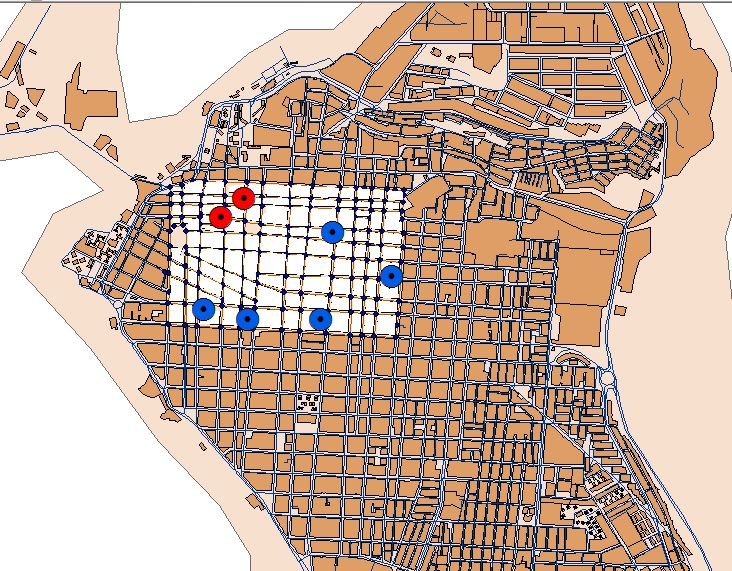
\includegraphics[scale=0.44]{Figuras/mapa2.jpg} 
	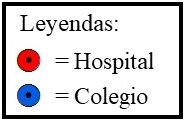
\includegraphics[scale=0.5]{Figuras/simb1.jpg}
	\caption{Extracto de la zona. Fuente: Elaboración propia.}
	\label{fig:fig4}
\end{figure}

\begin{figure}[h!]
	\centering
	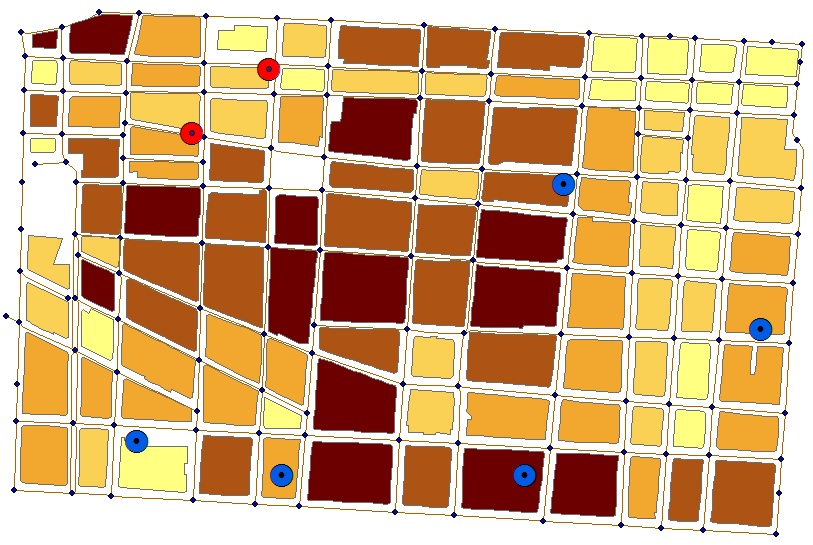
\includegraphics[scale=0.4]{Figuras/mapa1.jpg}
	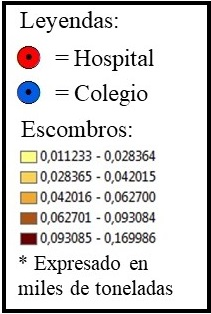
\includegraphics[scale=0.5]{Figuras/simb3.jpg} 
	\caption{Detalle del extracto de la zona con cantidad de escombros. Fuente: Elaboración propia.}
	\label{fig:fig5}
\end{figure}

\pagebreak

\subsubsection{Escenarios propuestos}

La ejecución del modelo se proponen siete escenarios, los cuales se detallan a continuación:

\begin{itemize}
	\item Escenario 0: Escenario Base.
	\item Escenario 1: Sin considerar el ponderador de prioridad.
	\item Escenario 2: 5 camiones operativos.
	\item Escenario 3: 15 camiones operativos.
	\item Escenario 4: Aumento del 10 \% volumen de escombros.
	\item Escenario 5: Aumento del 20 \% volumen de escombros.
	\item Escenario 6: Aumento del 30 \% volumen de escombros.
\end{itemize}

El Escenario 0 se analiza la situación actual, considerando una flota homogénea de 10 vehículos, 7 vueltas y un horizonte de planificación de 5 días. En el escenario 1 se analizan los resultados sin el factor de prioridad, para comparar su impacto. En los escenarios 2 y 3 se disminuye y aumenta el nivel en la flota, respectivamente. Por último, en los escenarios 4, 5 y 6 se analiza la variación aumentando los niveles en los volúmenes de escombros en 10\%, 20\% y 30\%, respectivamente.


\section{Análisis de la situación inicial (Escenario 0)}

En la situación actual, al considerar un terremoto de 8.0 Mw de magnitud, se obtienen los resultados de la Tabla \ref{tab:tab2}

\begin{table*}[h!]
\resizebox{18cm}{!} {
\begin{tabular}{c|c|c|c|c|c|c|c|c|c}
\hline
\multirow{3}{*}{Escenario} & Función                   & Tiempo & GAP                   & Edificios                & Cant. prom. de                 & No. prom. de días & \multicolumn{3}{c|}{Cant. de días promedio de limpieza}                          \\ \cline{8-10} 
                           & \multirow{2}{*}{objetivo} & CPU    & \multirow{2}{*}{(\%)} & \multirow{2}{*}{Limpios} & escombros recolectados         & para limpiar      & \multirow{2}{*}{Hospitales} & \multirow{2}{*}{Colegios} & \multirow{2}{*}{Otros} \\
                           &                           & (seg)  &                       &                          & por día $M^{3}$ & un edificio       &                             &                           &                        \\ \hline
0                          & 103                       & 18000  & 1.33                  & 108                      & 1,254.97                         & 2.26              & 1                           & 1                         & 1.67                   \\ \hline
\end{tabular}
}
\caption{Detalle de modelamiento Escenario 0, Fuente: Elaboración propia.}
\label{tab:tab2}
\end{table*}

%%%%%%%%%%%%%%%%%%%%%%%%%%%%%%%%%%%%%%%%%%%%%%%%%%%%%%%%%%%%%%%%%%%%%%%%%%%

%Arreglar la tabla para que quepa aquí, y poner los títulos correspondientes con letras

%%%%%%%%%%%%%%%%%%%%%%%%%%%%%%%%%%%%%%%%%%%%%%%%%%%%%%%%%%%%%%%%%%%%%%%%%%%%%

El modelo matemático se ejecutó por 5 horas, obteniendo un GAP del $1.33\%$. En esta instancia, se limpiaron 108 edificios, la cantidad de escombros recolectada es 3.761,23 $m^{3}$ .
En la Figura \ref{fig:esc0-graf} se presenta el gráfico de la cantidad de edificios limpiados por día, donde se aprecia que, a medida que pasan los días, se limpia una menor cantidad de edificios. Esto se justifica debido a que se le da prioridad al primer día de limpiar la mayor cantidad de nodos. Además se puede destacar que el modelo propuesto solo utilizó 3 días de los 5 propuestos en el horizonte de planificación.


%%%%%%%%%%%%%%%%%%%%%%%%%%%%%%%%%%%%%%%%%%%%%%%%%%%%%%%%%%%%%%%%%%%%%%%%%%%

\begin{figure}[h!]
\centering
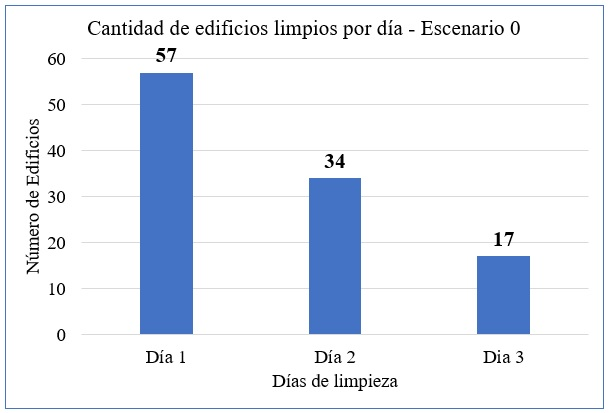
\includegraphics[scale=0.7]{Figuras/INDIC1.jpg} 
\caption{Detalle de edificios limpios (Escenario 0), Fuente: Elaboración propia}
\label{fig:esc0-graf}
\end{figure}

%%%%%%%%%%%%%%%%%%%%%%%%%%%%%%%%%%%%%%%%%%%%%%%%%%%%%%%%%%%%%%%%%%%%%%%%%%%%%

La distribución espacial de limpieza de los edificios se ve representada en la Figura \ref{fig:esc0-visu}, donde se visualiza cómo se van limpiando los edificios a medida que pasan los días. Aquí se observa la representación del factor de preferencia, limpiando una mayor cantidad de edificios el día 1 que al termino de los días de limpieza.


%%%%%%%%%%%%%%%%%%%%%%%%%%%%%%%%%%%%%%%%%%%%%%%%%%%%%%%%%%%%%%%%%%%%%%%%%%%

\begin{figure}[h!]
\centering
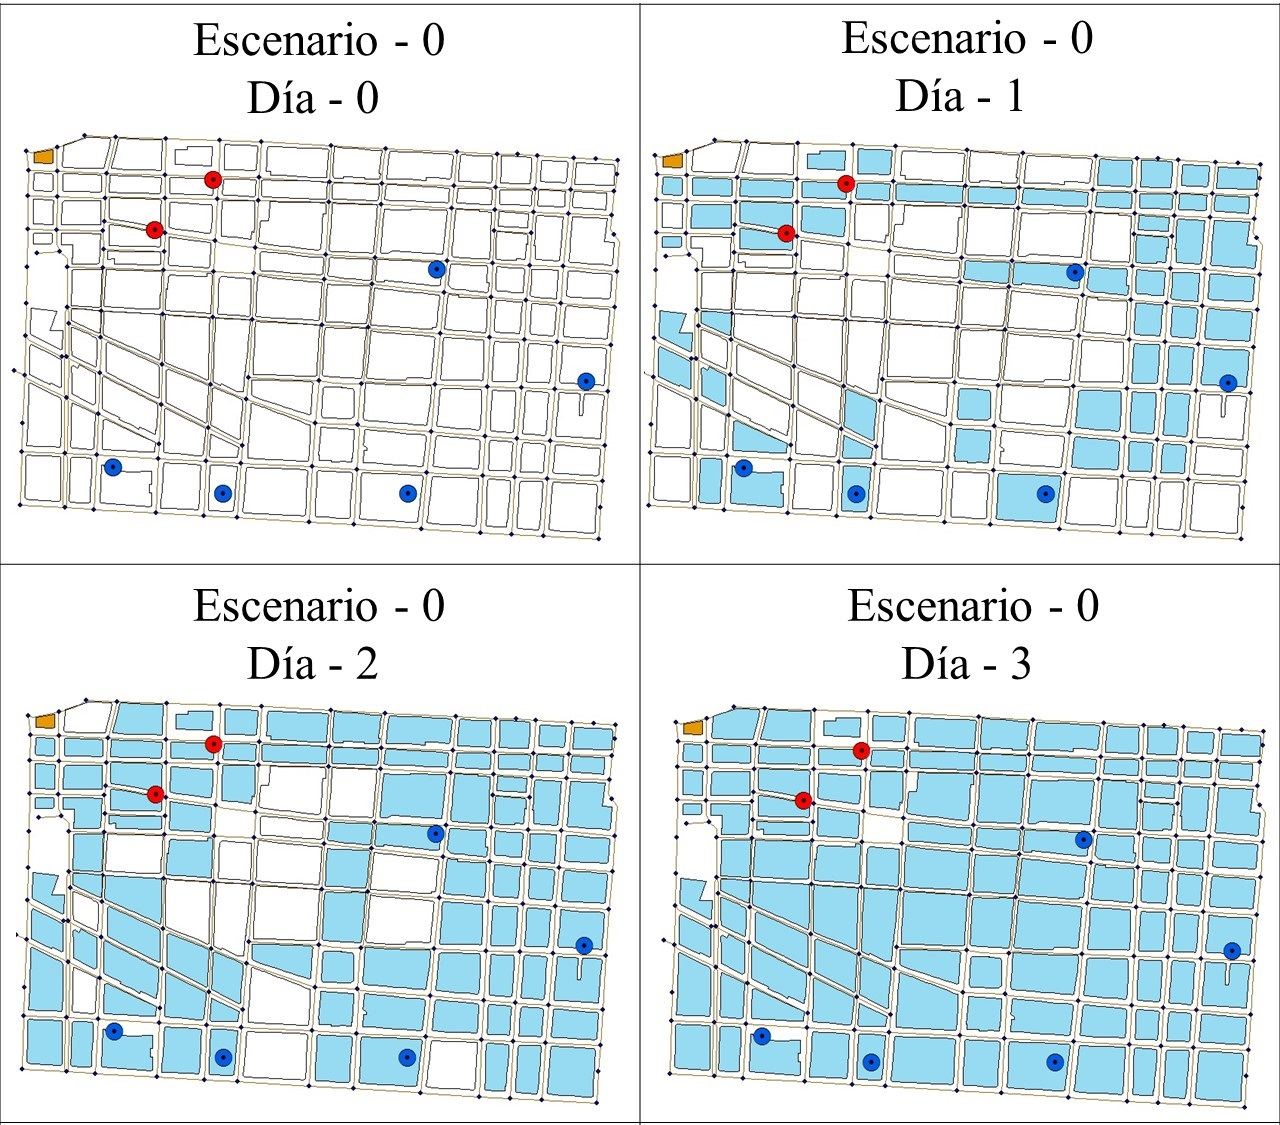
\includegraphics[scale=0.25]{Figuras/visu1.jpg}
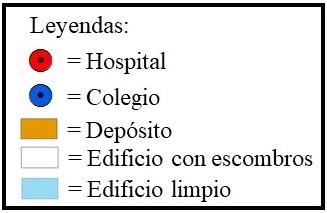
\includegraphics[scale=0.45]{Figuras/simb2.jpg} 
\caption{Visualización de edificios limpios  (Escenario 0), Fuente: Elaboración propia}
\label{fig:esc0-visu}
\end{figure}

%%%%%%%%%%%%%%%%%%%%%%%%%%%%%%%%%%%%%%%%%%%%%%%%%%%%%%%%%%%%%%%%%%%%%%%%%%%%%

En resumen, del escenario 0 se puede concluir que el modelo sí realiza una priorización exitosa al considerar los ponderadores de tipo de edificio y día, puesto que en la Figura \ref{fig:esc0-graf} se muestra cómo se agrupa la mayor cantidad de edificios en los primeros días y en la Figura \ref{fig:esc0-visu} que los primeros en limpiarse son los de mayor prioridad y luego los que presentan mayores escombros. Asimismo, mediante los indicadores se vuelve a verificar el coeficiente de prioridad limpiando los hospitales y colegios en el primer día de trabajo.


\section{Análisis de la metodología sin factor de preferencia (Escenario 1)}

En este análisis se detalla cómo se comporta el modelo sin los factores de preferencia. En la Tabla \ref{tab:comp01} se muestran los resultados.


%%%%%%%%%%%%%%%%%%%%%%%%%%%%%%%%%%%%%%%%%%%%%%%%%%%%%%%%%%%%%%%%%%%%%%%%%%%

\begin{table*}[h!]
\resizebox{18cm}{!} {
\begin{tabular}{c|c|c|c|c|c|c|c|c|c}
\hline
\multirow{3}{*}{Escenario} & Función                   & Tiempo & GAP                   & Edificios                & Cant. prom. de                 & No. prom. de días & \multicolumn{3}{c|}{Cant. de días promedio de limpieza}                          \\ \cline{8-10} 
                           & \multirow{2}{*}{objetivo} & CPU    & \multirow{2}{*}{(\%)} & \multirow{2}{*}{Limpios} & escombros recolectados         & para limpiar      & \multirow{2}{*}{Hospitales} & \multirow{2}{*}{Colegios} & \multirow{2}{*}{Otros} \\
                           &                           & (seg)  &                       &                          & por día m\textasciicircum{}(3) & un edificio       &                             &                           &                        \\ \hline
0                          & 103                       & 18000  & 1.33                  & 108                      & 1,254.97                       & 2.26              & 1                           & 1                         & 1.67                   \\ 
1                          & 117                       & 40     & 0.00                  & 108                      & 752.25                         & 2.26              & 2.53                        & 3                         & 2.5                    \\ \hline
\end{tabular}
}
\caption{Detalle comparación Escenarios 0 y 1, Fuente: Elaboración propia. }
\label{tab:comp01}
\end{table*}

%%%%%%%%%%%%%%%%%%%%%%%%%%%%%%%%%%%%%%%%%%%%%%%%%%
El modelo matemático se ejecutó por 40 segundos, obteniendo un GAP del $0.00\%$ debido que al quitar el factor de preferencia se simplifica ejecutar el modelamiento. En esta instancia, al igual que en la anterior se limpiaron 108 edificios y la cantidad de escombros recolectada es 3.761,23 $m^{3}$.

En la Figura \ref{fig:esc01graf} se presenta el gráfico de la cantidad de edificios limpiados por día, donde se aprecia que, al eliminar el factor de preferencia se realiza una limpieza constante, distinto lo que hace el escenario 0. Además se puede confirmar la limpieza contante a causa de la utilización de los 5 días del horizonte de planificación. Asimismo mediante los indicadores, se verifica una menor cantidad de escombros recolectados por día, destacando un rendimiento uniforme durante el horizonte de planificación.


\begin{figure}[h!]
\centering
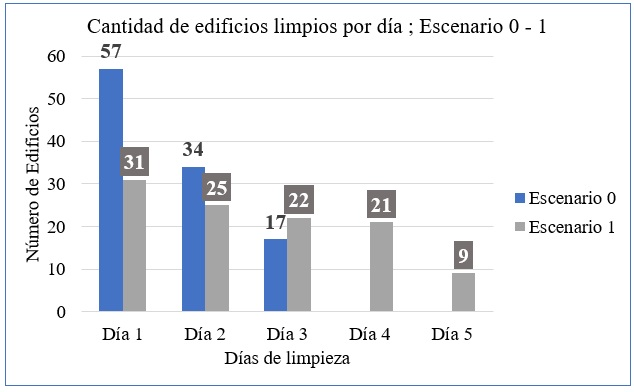
\includegraphics[scale=0.65]{Figuras/INDIC2.jpg} 
\caption{Detalle de edificios limpios (Escenarios 0 y 1), Fuente: Elaboración propia}
\label{fig:esc01graf}
\end{figure}



%%%%%%%%%%%%%%%%%%%%%%%%%%%%%%%%%%%%%%%%%%%%%%%%%%
La distribución espacial de limpieza de los edificios se ve representada en la Figura \ref{fig:esc01-visu}, donde se visualiza cómo se van limpiando los edificios a medida que pasan los días. Aquí se observa la comparación de los primeros 3 días del horizonte de planificación demostrando la limpieza constante versus el comportamiento de la limpieza con el factor de preferencía de limpieza hacia los primeros días de trabajo.


\begin{figure}[h!]
\centering
\includegraphics[scale=0.25]{Figuras/visu2.jpg} 
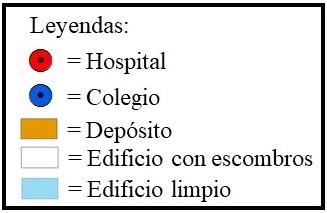
\includegraphics[scale=0.45]{Figuras/simb2.jpg}
\caption{Visualización de edificios limpios  (Escenarios 0 y 1), Fuente: Elaboración propia}
\label{fig:esc01-visu}
\end{figure}


%%%%%%%%%%%%%%%%%%%%%%%%%%%%%%%%%%%%%

En resumen, del escenario 1 se puede concluir que el modelo realiza un rendimiento constante en cuanto a limpieza puesto que en la Figura \ref{fig:esc01graf} se muestra una comparación del horizonte de planificación, representando un número de limpieza constante en el escenario 1 y la priorización de la limpieza hacia los primeros días en el escenario 0. Además en la Figura \ref{fig:esc01-visu} se realiza la comparación respectiva de los primeros 3 días del horizonte de planificación, donde representa la falencía en la limpieza del escenario 1. Asimismo, mediante los indicadores se puede comprobar que la variación afecta directamente a la prioridad de limpiar Hospitales y colegios, aumentando considerablemente el tiempo en habilitar los edificios mencionados.

%%%%%%%%%%%%%%%%%%%%%%%%%%%%%%%%%%%%%%%%%%

%Presentarla igual que en el primer escenario, sin números, mostrando solo los indicadores que te mostré. Luego explicar y mostrar el gráfico de la comparación de escenarios 0 y 1. Terminas con la figura de los 4 mapas, explicando de la misma manera que lo hcie en 1.

%%%%%%%%%%%%%%%%%%%%%%%%%%%%%%%%%%%%%%%%%%%%%%%%%%%%%%%%%%%%%%%%%%%%%%%%%%%%%

\section{Análisis de variación en el recurso vehicular (Escenarios 2 y 3)}

En este análisis se detalla cómo se comporta el modelo variando la cantidad de vehículos operativos. En la Tabla \ref{tab:comp02} se muestran los resultados.
\begin{table*}[h!]
\resizebox{18cm}{!} {
\begin{tabular}{c|c|c|c|c|c|c|c|c|c}
\hline
\multirow{3}{*}{Escenario} & Función                   & Tiempo & GAP                   & Edificios                & Cant. prom. de                 & No. prom. de días & \multicolumn{3}{c|}{Cant. de días promedio de limpieza}                          \\ \cline{8-10} 
                           & \multirow{2}{*}{objetivo} & CPU    & \multirow{2}{*}{(\%)} & \multirow{2}{*}{Limpios} & escombros recolectados         & para limpiar      & \multirow{2}{*}{Hospitales} & \multirow{2}{*}{Colegios} & \multirow{2}{*}{Otros} \\
                           &                           & (seg)  &                       &                          & por día m\textasciicircum{}(3) & un edificio       &                             &                           &                        \\ \hline
0                          & 103                       & 18000  & 1.33                  & 108                      & 1,254.97                       & 2.26              & 1                           & 1                         & 1.67                   \\ 
2                          & 78                        & 18000  & 7.21                  & 99                       & 658.34                         & 1.99              &  1                       & 1.4                          & 2.57                   \\
3                          & 109                       & 18000  & 1.48                  & 107                      & 1,863.41                       & 2.24              & 1                           & 1                         & 1.32                   \\ \hline
\end{tabular}
}
\caption{Detalle comparación Escenarios 0, 2 y 3, Fuente: Elaboración propia. }
\label{tab:comp02}
\end{table*}

%%%%%%%%%%%%%%%%%%%%%%%%%%%%%%%%%%%%%%%%

Ambos modelos matemáticos de los escenarios 2 y 3 se ejecutaron por 5 horas, obteniendo un GAP de $7.21\%$ y $1.48\%$ respectivamente. En estas instancias, se limpiaron 99 y 107 edificios y  la cantidad de escombros recolectada es de  3.291,71 $m^{3}$  y  3.726,81 $m^{3}$ respectivamente.
En la Figura \ref{fig:esc023-graf} se presenta el gráfico de la cantidad de edificios limpiados por día, donde se aprecia que, existe dificultad de trabajar con 5 camiones en el escenario 2 y la facilidad del escenario 3 en cumplir el objetivo de realizar la limpieza global en solo 2 días, debido que cuenta con 15 camiones operativos. Además se puede destacar que los modelos propuestos utilizaron de excelente manera los recursos proporcionados, limpiando los edificios de mayor prioridad en el primer día del horizonte de  planificación.

%%%%%%%%%%%%%%%%%%%%%%%%%%%%%%%%%%%%%%%%%%%%


\begin{figure}[h!]
\centering
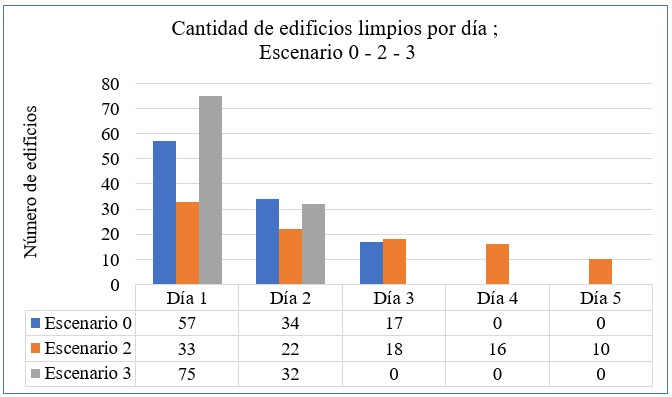
\includegraphics[scale=0.63]{Figuras/INDIC3.jpg} 
\caption{Detalle de edificios limpios (Escenarios 0, 2 y 3), Fuente: Elaboración propia}
\label{fig:esc023graf}
\end{figure}

%%%%%%%%%%%%%%%%%%%%%%%%%%%%%%%%%


La distribución espacial de limpieza de los edificios se ve representada en la Figura \ref{fig:esc023-visu}, donde se visualiza cómo se van limpiando los edificios a medida que pasan los 2 primeros días de trabajo. Aquí se observa la comparación de los edificios completamente limpios durante el horizonte de planificación de los 3 escenarios, representando la diferencia en cuanto a proporción de recursos utilizados, presentando un deficit de cantidad de edificios limpios en el escenario 2 y una ventaja en cuanto a la limpieza de edificios en el escenario 3 ambos siendo comparados con el escenario 0.

\begin{figure}[h!]
\centering
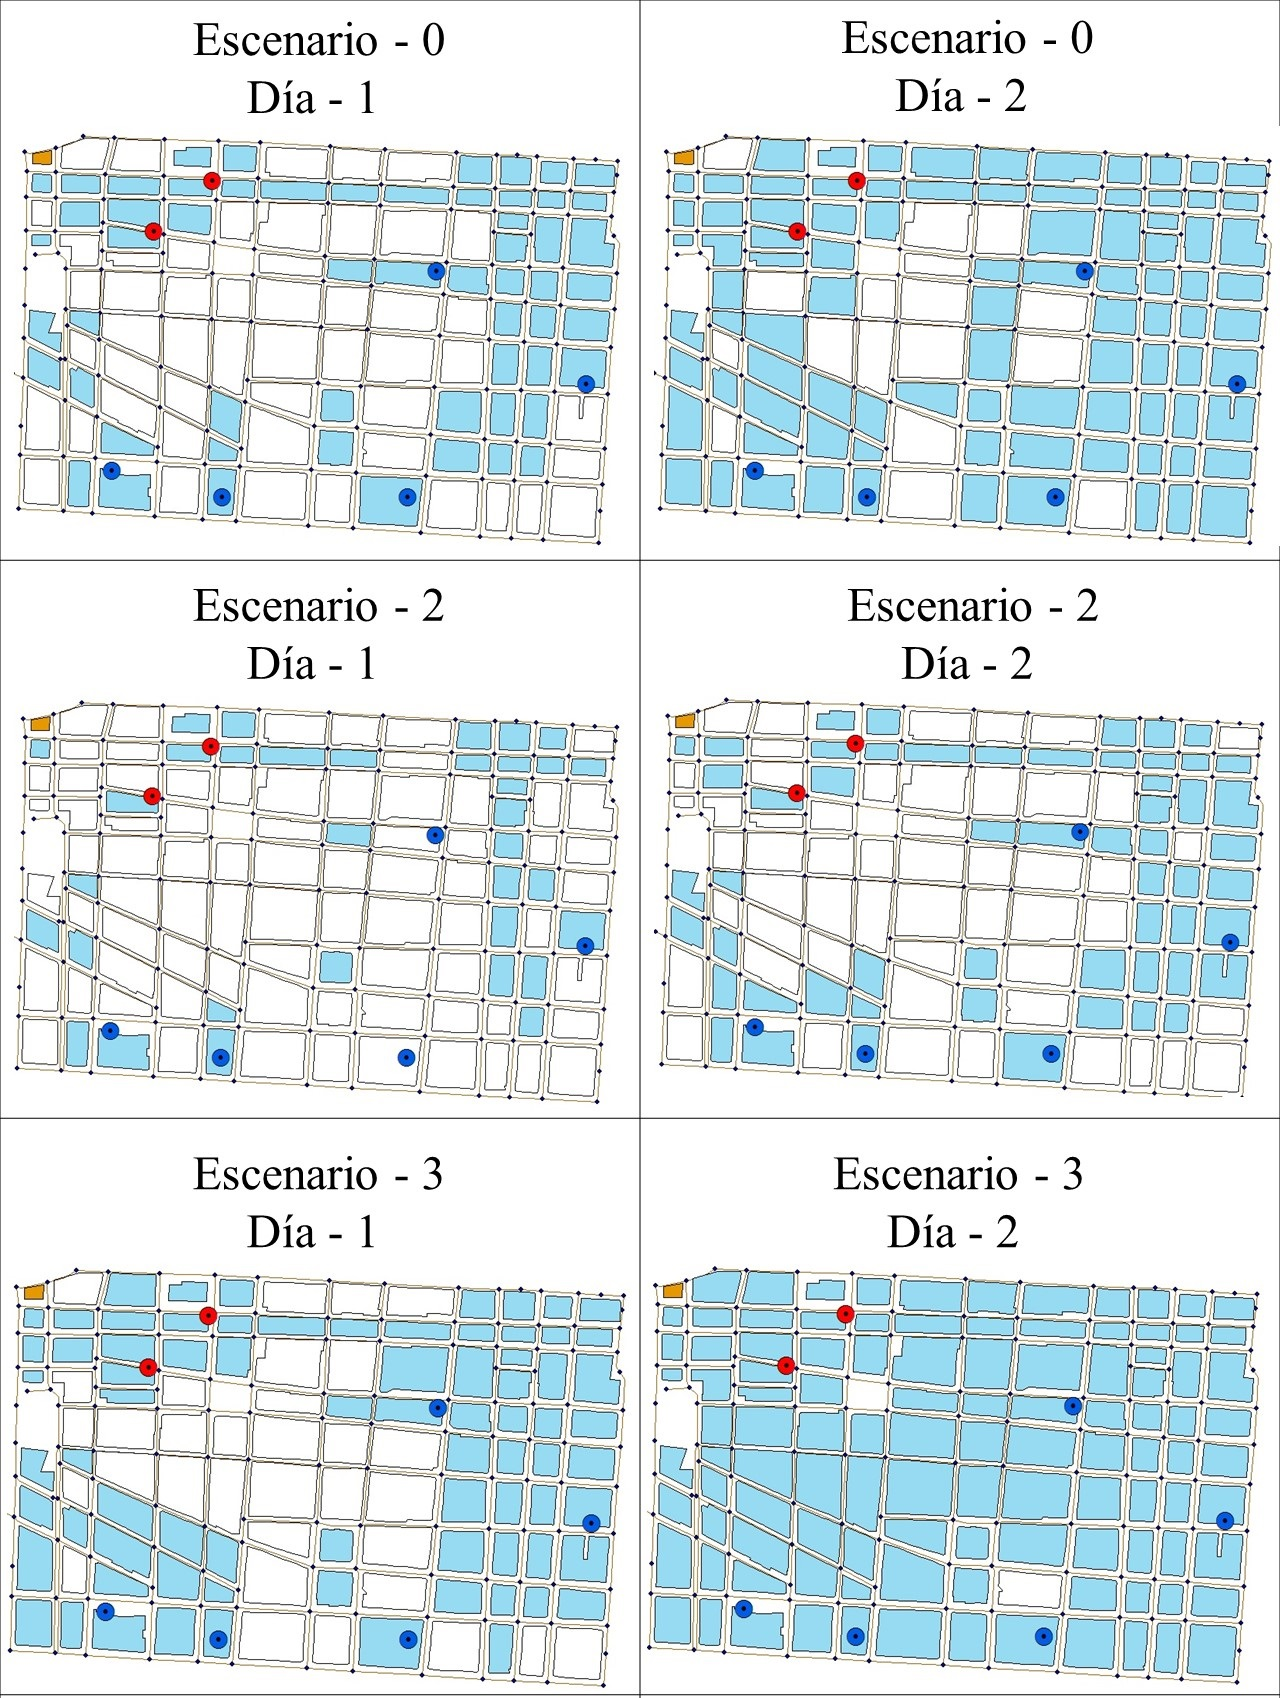
\includegraphics[scale=0.26]{Figuras/visu3.jpg} 
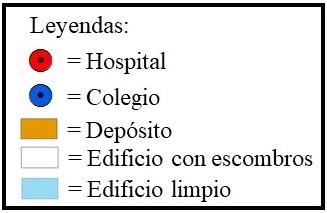
\includegraphics[scale=0.45]{Figuras/simb2.jpg} 
\caption{Visualización de edificios limpios  (Escenarios 0, 2 y 3), Fuente: Elaboración propia}
\label{fig:esc023-visu}
\end{figure}
	
%%%%%%%%%%%%%%%%%%%%%%%%%%%%%%%%%%%%%%

En resumen, de los escenarios 2 y 3 se puede concluir que los modelos si realizan una priorización exitosa de los ponderadores de tipo de edificio y día, puesto que en la Figura \ref{fig:esc023graf} se muestra una comparación del horizonte de planificación, representando la priorización de limpieza en el primer día del horizonte de planificación. Además en la Figura \ref{fig:esc023-visu} se realiza la comparación respectiva de los primeros 2 días del horizonte de planificación, donde representa la importancia de contar con los recursos suficientes para realizar los trabajos respectivos de limpieza. Asimismo, mediante los indicadores se puede comprobar que la variación no afecta la priorización de limpieza de los edificios tales como Hospitales y colegios.

\section{Análisis de variación en la cantidad de escombros (Escenarios 4, 5 y 6)}

En este análisis se detalla cómo se comporta el modelo aumentando la cantidad de volumen de escombros de cada edificio. En la Tabla \ref{tab:comp03} se muestran los resultados.

\begin{table*}[h!]
\resizebox{18cm}{!} {
\begin{tabular}{c|c|c|c|c|c|c|c|c|c}
\hline
\multirow{3}{*}{Escenario} & Función                   & Tiempo & GAP                   & Edificios                & Cant. prom. de                 & No. prom. de días & \multicolumn{3}{c|}{Cant. de días promedio de limpieza}                          \\ \cline{8-10} 
                           & \multirow{2}{*}{objetivo} & CPU    & \multirow{2}{*}{(\%)} & \multirow{2}{*}{Limpios} & escombros recolectados         & para limpiar      & \multirow{2}{*}{Hospitales} & \multirow{2}{*}{Colegios} & \multirow{2}{*}{Otros} \\
                           &                           & (seg)  &                       &                          & por día m\textasciicircum{}(3) & un edificio       &                             &                           &                        \\ \hline
0                          & 103                       & 18000  & 1.33                  & 108                      & 1,254.97                       & 2.26              & 1                           & 1                         & 1.67                   \\ 
4                          & 99                        & 18.000 & 3.83                  & 104                      & 1.204,30                       & 2.29              & 1                           & 1.2                       & 1.69                   \\ 
5                          & 98                        & 18.000 & 2.65                  & 106                      & 738.44                         & 2.59              & 1                           & 1.2                       & 1.83                   \\ 
6                          & 96                        & 18.000 & 2.34                  & 106                      & 926.04                         & 2.75              & 1                           & 1.2                       & 1.92                   \\ \hline
\end{tabular}
}
\caption{Detalle comparación Escenarios 0, 4, 5 y 6 Fuente: Elaboración propia. }
\label{tab:comp03}
\end{table*}

%%%%%%%%%%%%%%%%%%%%%%%%%%%%%%%%%%%%%%%%%%%%

Los 3 modelos matemáticos de los escenarios 4, 5 y 6 se ejecutaron por 5 horas, obteniendo un GAP de $3.83\%$, $2.65\%$ y $2.34\%$ respectivamente. En estas instancias, se limpiaron 104 edificios en el escenario 4 y 106 edificios en los escenarios 5 y 6. La cantidad de escombros recolectada es de  3,612.89 $m^{3}$, 3.692,21 $m^{3}$  y  3.704,18 $m^{3}$ respectivamente.
En la Figura \ref{fig:esc0456graf} se presenta el gráfico de la cantidad de edificios limpiados por día, donde se aprecia que, al aumentar la cantidad de volumen de escombros por edificio, se presenta una menor cantidad de edificios limpios en comparación al escenario 0 y a la vez se puede visualizar la priorización correcta, de limpieza de los edificios hacia los primeros días del horizonte de planificación siendo comprobado por la cantidad de edificios completamente limpios en los primeros 3 días de trabajo.


%%%%%%%%%%%%%%%%%%%%%%%%%%%%%%%%%%%%%%%%%%%%%%%%%%%%%%%%%%%%%%%%%%%%%%%%%%%
\begin{figure}[h!]
\centering
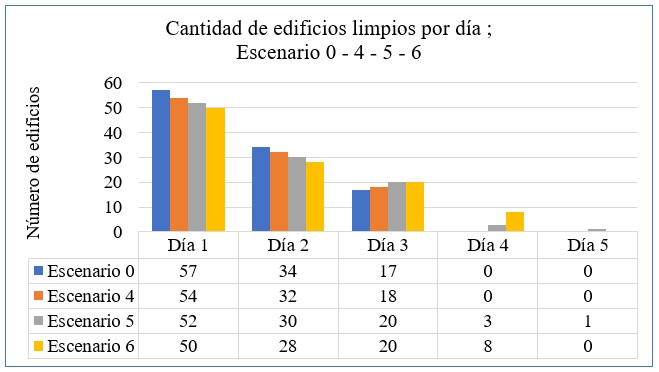
\includegraphics[scale=0.63]{Figuras/INDIC4.jpg} 
\caption{Detalle de edificios limpios (Escenarios 0, 4, 5 y 6), Fuente: Elaboración propia}
\label{fig:esc0456graf}
\end{figure}


%%%%%%%%%%%%%%%%%%%%%%%%%%%%

La distribución espacial de limpieza de los edificios se ve representada en la Figura \ref{fig:esc0456-visu}, donde se visualiza cómo se van limpiando los edificios durante el primer y tercer día de trabajo. Aquí se observa la comparación de los edificios completamente limpios durante el horizonte planificación de los 4 escenarios, representando como aumenta la dificultad al incrementar el volumen de escombros por edificio, presentando una visualización del decrecimiento de edificios completamente limpio en cada escenario respectivo.

\begin{figure}[h!]
\centering
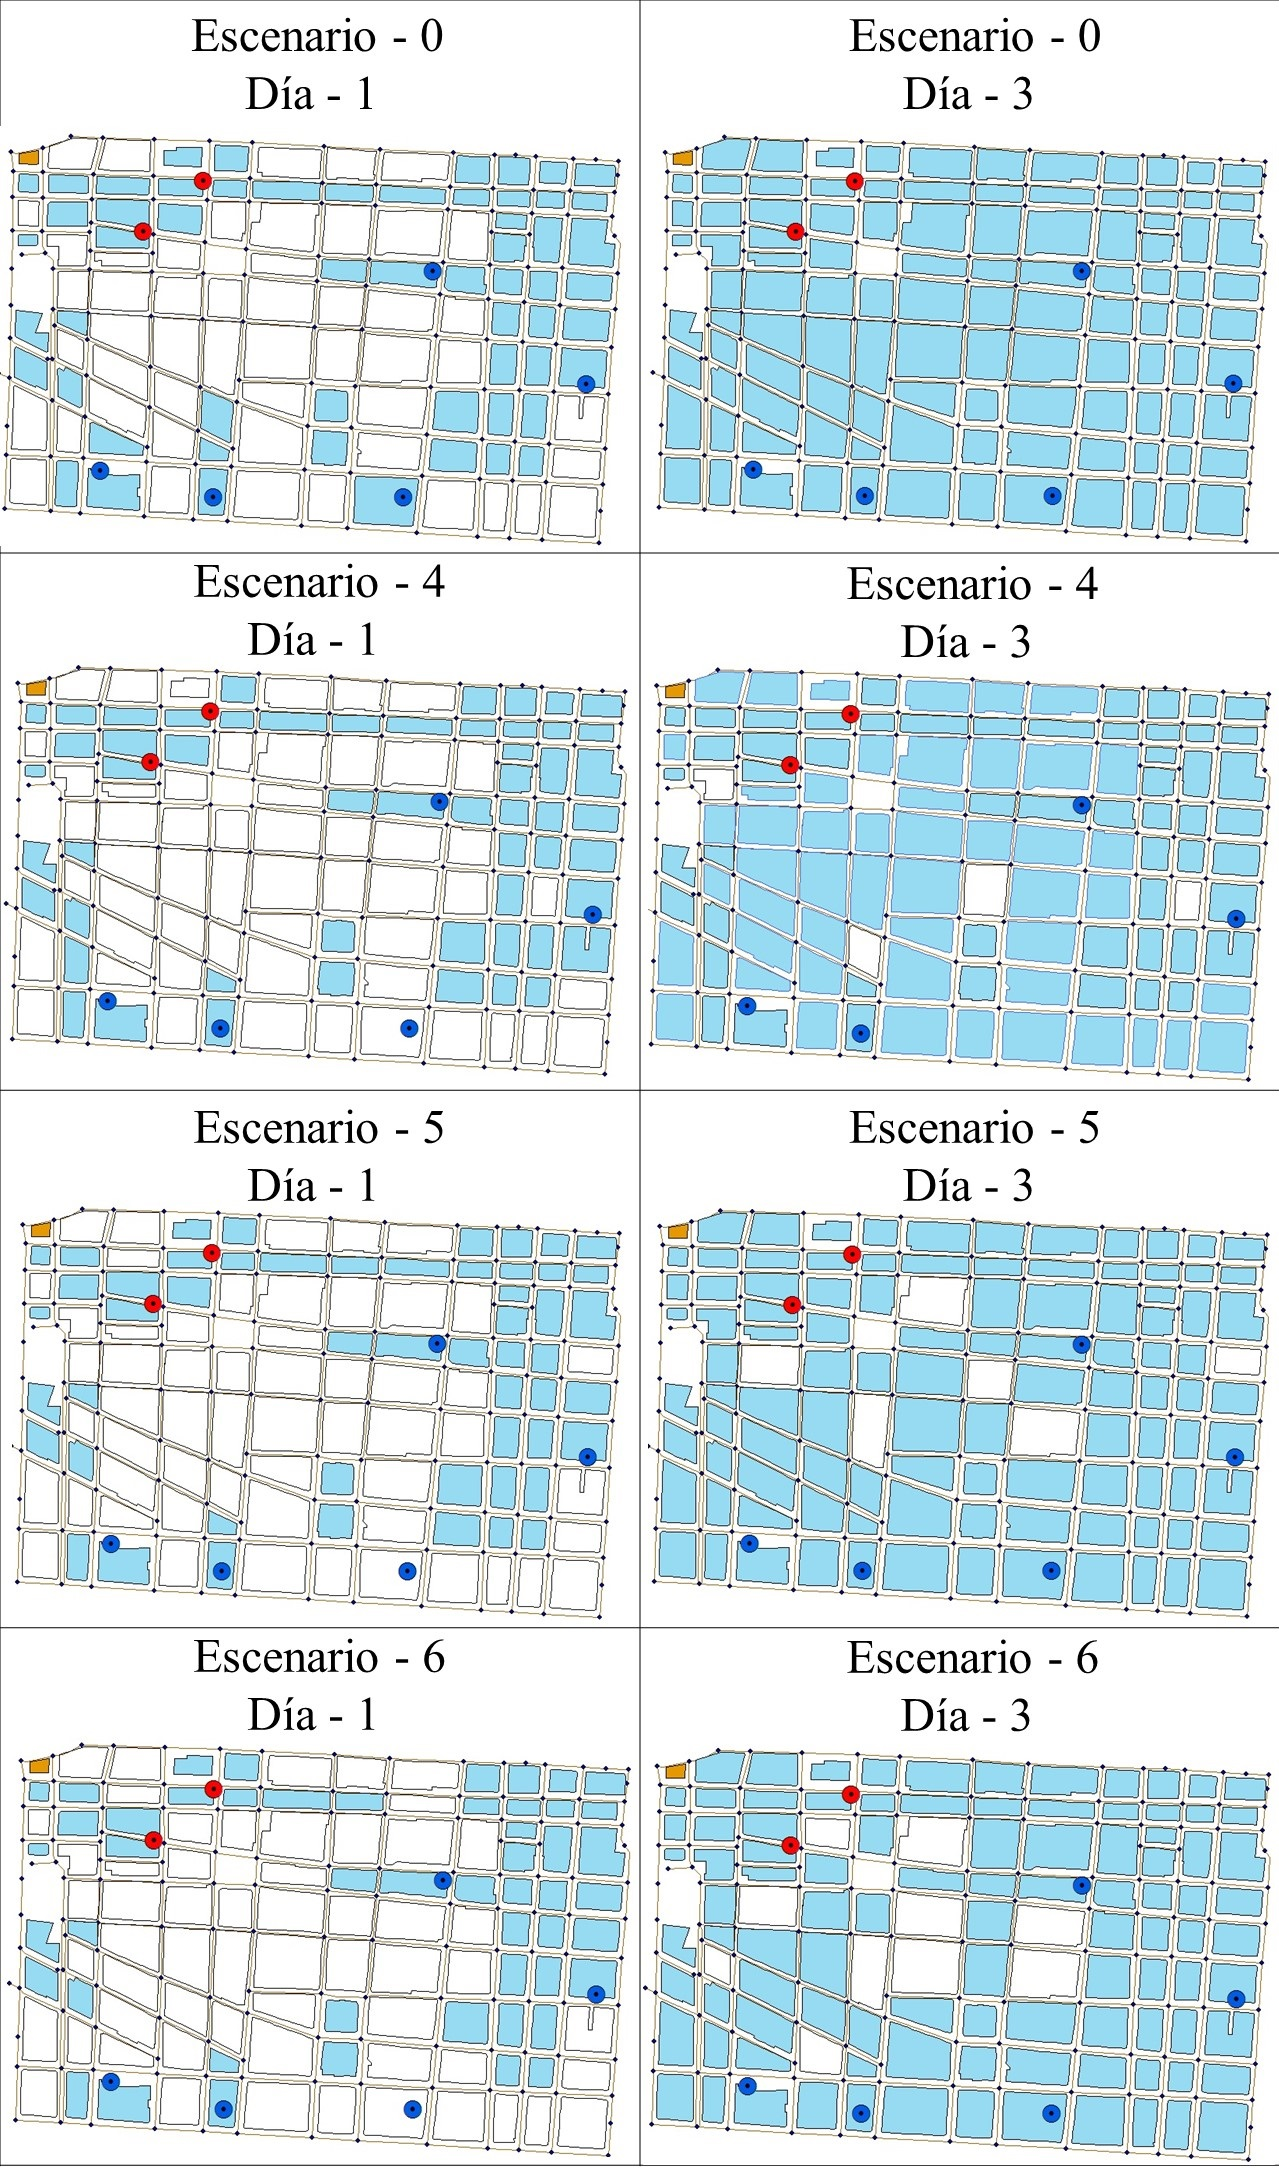
\includegraphics[scale=0.25]{Figuras/visu4.jpg}
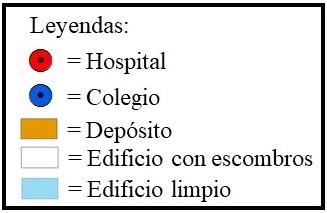
\includegraphics[scale=0.45]{Figuras/simb2.jpg}  
\caption{Visualización de edificios limpios  (Escenarios 0, 2 y 3), Fuente: Elaboración propia}
\label{fig:esc0456-visu}
\end{figure}

%%%%%%%%%%%%%%%%%%%%%%%%%%%%%%
\pagebreak

En resumen, de los escenario 4, 5 y 6 se puede concluir que los  modelos si realizan una priorización exitosa de los ponderadores de tipo de edificio y día, puesto que en la Figura \ref{fig:esc0456graf} se muestra una comparación del horizonte de planificación, representando la priorización de limpieza en el primer día del horizonte de planificación. Además en la Figura \ref{fig:esc0456-visu} se realiza la comparación respectiva de los primer y tercer día del horizonte de planificación, donde representa dificultad de realizar la limpieza al aumentar el volumen de escombros, disminuyendo considerablemente el numero de edificios completamente limpio. Además mediante los indicadores, se verifica que el modelo responde correctamente a la priorización de limpieza de los edificios en el primer día de trabajo.

%%%%%%%%%%%%%%%%%%%%%%%%%%%%%

%Una vez que terminas de rellenar todo esto, es lo mismo en el paper y en la PPT.

%%%%%%%%%%%%%%%%%%%%%%%%%%%%%%%%%%%%%%%%%%%%%%%%%%%%%%%%%%%%%%%%%%%%%%%%%%%%%

\section{CONCLUSIÓN Y TRABAJOS FUTUROS}

En esta investigación se desarrolló una metodología que permite tomar decisiones tácticas y operativas, puesto que es capaz de planificar la asignación de recursos claves posterior de ocurrir un desastre natural y dentro de un horizonte de planificación. Además, el modelo realiza consideraciones de elementos como capacidad de carga de camión, volumen de escombros por edificio, distribución espacial de los edificios con prioridad de estar completamente limpios.  Asimismo, considera el objetivo de realizar la preferencia de limpieza de los edificios hacia los primeros días del horizonte de planificación, además de priorizar los edificios que más ayudan a la población en el caso de un desastre, los cuales son los hospitales y centros de educación.

Posteriormente, se comprueba el modelo propuesto en un escenario base, en una instancia menor a la totalidad de la ciudad propuesta en el caso de estudio, con características experimentales tales como número de camiones, número de vueltas y número de días. Consecutivamente, se realiza diversos análisis de variación del escenario base, presentando variaciones en quitar el factor de preferencia, variar la cantidad de camiones operativos y aumentar la cantidad de volumen de escombros. 

Los resultados de cada escenario propuesto fueron comparados con el escenario base, para verificar cómo se comporta el modelo y comprobar que la cantidad de edificios completamente limpios no afecte en el objetivo general, limpiando la mayor cantidad de edificios hacia los primeros días del horizonte de planificación. Los resultados en general se consideran favorables para la modelación, a causa de que la mayoría de los modelos limpia favorablemente los edificios con priorización, es decir hospitales y colegios.

Si bien el problema se puede resolver computacionalmente en un tiempo razonable, cuando se tiene una instancia mayor presenta prolongados tiempos de computo, por lo cual en un trabajo a futuro se podría presentar una heurística que permita desarrollar resultados en menores tiempos de modelación. A la vez se debería considerar incluir el rendimiento de bulldozer para obtener tiempos en la operación completa y finalmente completando el equipo de limpieza con la inclusión de una retroexcavadora para remover los materiales distintos de madera y ladrillos. También para obtener un mejor provecho de la remoción de escombros en general, se podría considerar algún tipo de zonas de almacenamiento temporal, ya sean plazas y/o terrenos sin habitantes ni construcciones, para poder recolectar de manera provisional escombros, cuyo beneficio se reflejaría en el tiempo de transito de los camiones recolectores. En esté caso no se menciona aspectos de reciclajes, por lo cual se consideraría una desventaja al largo plazo, es importante incluir los equipos que podrían realizar reciclaje para reutilizar los materiales de construcción.  Asimismo, se deberían considerar múltiples depósitos para gestionar una mayor capacidad de escombros, en el mejor caso agregar un parámetro de generación de depósitos de ser necesario. Finalmente, se debería incorporar el traslado de escombros entre nodos para agilizar la habilitación de los edificios con mayor priorización tales como hospitales, colegios y albergues.















%\section{Caso de estudio}
%
%\subsection{Área de estudio}
%
%El caso de estudio se realizó en la región de Tarapacá en la ciudad de Iquique, Chile, visualizada en la Figura \ref{fig:fig1}. Esta ciudad cuenta con una población de 191.468 personas y una superficie de 2.262,4 $m^{2}$ \citep{CENSO2017}.
%
%\begin{figure}[h!]
%\centering
%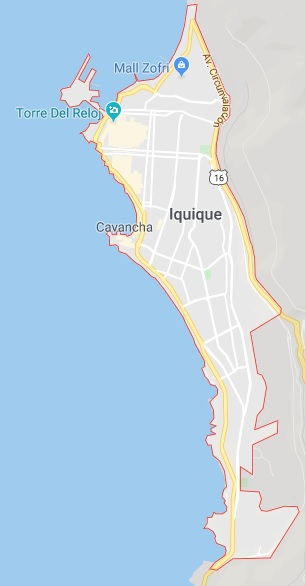
\includegraphics[scale=0.4]{Figuras/iquique1.jpg}
%\caption{Mapa de Iquique. Fuente: Google Maps (2019)}
%\label{fig:fig1}
%\end{figure}
%
%Esta región está propensa a sufrir catástrofes naturales debido a su ubicación sobre la placa Sudamericana la cual produce un movimiento contrario a la placa de Nazca \citep{sismologia}. Según \citet{emdat}, se cuenta con un historial de cuatro sismos de gran magnitud en los últimos 25 años, debido a que superan los 7.0 grados de magnitud \citep{guc}.
%
%\subsection{Recopilación de datos}
%
%\subsubsection{Red vial y obtención de escombros}
%
%La red vial se obtuvo a través del Ministerio de Transporte y Telecomunicaciones de Chile, la cual se compone de 1655 manzanas censales \citet{CENSO2017}. Estos datos fueron procesados en el software ArcGis 10.1, del cual se obtuvo la matriz de distancia entre los nodos de la red.
%
%Por otro lado, la cantidad de escombros para cada una fue obtenida a través del software HAZUS 2.1, a partir de una simulación de un escenario de magnitud 8.0 Mw. Se tomó en consideración sólo los escombros de tipo madera y ladrillos, puesto que los demás requieren de equipamiento más avanzado \citep{hasuz}.
%
%\subsubsection{Edificios}
%
%Durante la fase de recuperación es importante mantener las vías de acceso despejadas a hospitales, colegios y otros edificios de interés. Estos se utilizan como recurso para la comunidad con el fin de albergar personas y/o prestar servicios de primeros auxilios \citet{lindell2006wiley}. En total se consideraron 16 centros de salud y 65 establecimientos de educación en la zona, cuya distribución se visualiza en la Figura \ref{fig:fig2} (Censo,2017)
%
%%%%%%%%%%%%%%%%%%%%%%%%%%%%%%%%%%%%%%%%%%%%%%%%%%%%%%%%%%%%%%
%
%%REF2 = pon la misma referencia que en la red vial.
%
%%%%%%%%%%%%%%%%%%%%%%%%%%%%%%%%%%%%%%%%%%%%%%%%%%%%%%%%%%%%%%%
%
%\begin{figure}[h!]
%	\centering
%	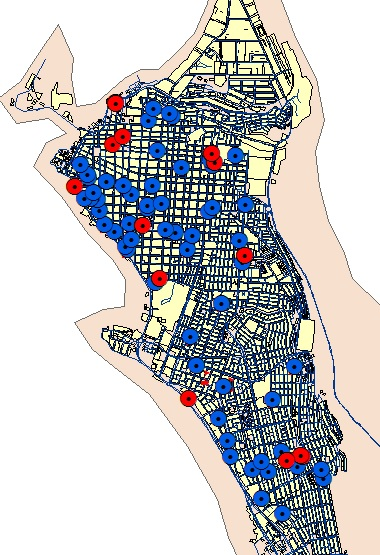
\includegraphics[scale=0.5]{Figuras/mapaarc.JPG}
%	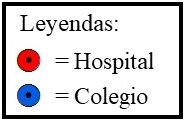
\includegraphics[scale=0.45]{Figuras/simb1.jpg}
%	\caption{Localidades de Iquique; Fuente: ArcGis 10.1 (2020)}
%	\label{fig:fig2}
%\end{figure}
%
%\subsubsection{Equipamiento vehicular}
%
%Durante las labores de recolección de escombros se necesitan equipos de limpieza, los cuales deben tener las capacitaciones necesarias para poder utilizar maquinaria pesada tal como bulldozers, vehículos livianos y camiones recolectores \citep{Kasaei2016}.
%
%El vehículo seleccionado es un camión IVECO modelo CAMIÓN TOLVA AD410 de potencia 420 HP y tracción 8x4. Se considera este camión transportador de escombros, el cual tiene una capacidad de transporte de 20 $m^3$ por viaje. Además, se considera una velocidad estándar de limpieza de $250 [m^{3}/h]$ \citep{Feng2003} y una velocidad de desplazamiento de $20000 [m/h]$. Finalmente, los vehículos cuentan con una capacidad de $4 m^{3}$ aproximadamente \citep{CAT}.
%
%\section{Resultados}
%
%
%
%
%
%
%
%
%
%
%
%
%
%
%
%
%
%
%Para realizar una demostración de los resultados, analizaremos de tres maneras distintas la información obtenida de los escenarios predefinidos. Los analisis serán presetandos mediante:
%\begin{itemize}
%	\item Cuadros.
%	\item Graficos.
%	\item Ilustraciones.
%\end{itemize}
%
%El escenario principal de la red de Iquique presentado en la figura \ref{FIGURA2}, fue obtenido mediante el software ArcGis 10.1, esté cuenta con aproximadamente 1.652 edificios, en donde se diferencian 16 Hospitales - Cesfam y 65 Colegios. 
%
%Con el objetivo de obtener resultados confiables, se generó un escenario de menor información a causa de generar distintos escenarios comparativos, cabe destacar que cada escenario fue simulado con el modelo propuesto por un tiempo de 5 horas continuas, debido a la complejidad del mismo.
%
%
%\subsection{INSTANCIA BASE - ESCENARIO 0}
%
%Se presenta con una posible catastrofe natural, generando una simulación a traves del software HAZUS de un potencial terremoto con una magintud de 8.0 Mw; generando información tal como: cantidad a escombros a remover por edificio y distancia entre los edificios. Cabe destacar que existe un nodo llamado punto de origen, que representa el punto de inicio y fin de cada vuelta en cada camión.
%
%El escenario 0, está conformado de 109 edificios con la cantidad de escombros expresada en $M^{3}$. La información presentada en la tabla adjunta de la figura \ref{Figura3}, está expresada en miles de toneladas, la información obtenida fue procesada para generar un calculo de la cantidad de escombros en $M^{3}$. Extrayendo la densidad de \cite{medida} 1.6  $Tons/m^{3}$
%
%\begin{figure}[h!]
%\centering
%\includegraphics[scale=0.45]{Figuras/arc1.jpg} \\
%\includegraphics[scale=0.75]{Figuras/arc2.jpg} 
%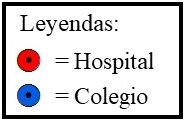
\includegraphics[scale=0.55]{Figuras/simb1.jpg} 
%\caption{Escenario - 0, Instancia base ; Fuente: Elaboración propia}
%\label{Figura3} 
%\end{figure}
%
%Se cuenta con 10 camiones recolectores de escombros con una capacidad de 20 $M^{3}$ y una velocidad constante de 30 $Km/H$, con una cantidad maxima de 7 vueltas dias en un horizonte de 5 días y 8 horas de trabajo diarias. \\
%% Se simulará 6 escenarios distintos, realizando variaciones en sus caracteristicas, con el objetivo de realizar comparativas con el escenario 0.
%
%\subsection{ESCENARIOS}
%
%Los escenarios presentandos a continuación estan simulados con igualdad de caracteristicas, solo presentan variaciones en factores claves, respecto al escenario base, con el objetivo de realizar comparaciones entre sí.
%
%\subsubsection{Escenario 1}
%
%La variación propuesta en esté escenario es quitar el ponderador de priodad, con el objetivo de analizar como se comportaría el modelo en caso de no presentar urgencias en la zona afectada.
%
%\subsubsection{Escenario 2 - 3}
%
%La variación propuesta en ambos escenarios, es alterar el numero de camiones respecto al escenario base, eliminando y agregando camiones a la jornada de trabajo, conformandose por  5 y 15 camiones operativos en cada escenario respectivo.
%
%\subsubsection{Escenario 4 - 5 - 6}
%La variación presentada en las ultimos tres escenarios, es aumentar el porcentaje de volumen de escombros por edificio, para generar una mayor  demanda en la carga de escombros, aumentando en $10\%$, $20\%$ y $30\%$, la cantidad de a extraer en cada escenario respectivo..
%
%
%\subsection{INDICADORES} 	
%Los indicadores obtenidos mediante las simulaciones realizadas se presentan en cuadro \ref{TABLA2}.
%
%\begin{table*}[h!]
%\resizebox{18cm}{!} {
%\begin{tabular}{c|c|c|c|c|c|c|c|c|c|c|c|c|c|c}
%\hline
%\multirow{2}{*}{Escenario} & \multirow{2}{*}{F0} & Tiempo CPU & \multirow{2}{*}{GAP} & Camiones   & Edificios & Utilización de & Escombros & \multirow{2}{*}{(1)} & \multirow{2}{*}{(2)} & \multirow{2}{*}{(3)} & \multirow{2}{*}{(4)} & \multirow{2}{*}{(5)} & \multirow{2}{*}{(6)} & \multirow{2}{*}{(7)} \\
%                           &                     & (segundos) &                      & operativos & limpios   & ponderador     & (\%)      &                      &                      &                      &                      &                      &                      &                      \\ \hline
%0                          & 103                 & 18.000     & 1,33\%               & 10         & 108       & Si             & 100\%     & 376,12               & 752,25               & 21,6                 & 2,26                 & 1,67                 & 1                    & 1                    \\ \hline
%1                          & 117                 & 40         & 0,00\%               & 10         & 108       & No             & 100\%     & 376,12               & 752,25               & 21,6                 & 2,26                 & 2,53                 & 3                    & 2,5                  \\ \hline
%2                          & 78                  & 18.000     & 7,21\%               & 5          & 99        & Si             & 100\%     & 694,43               & 694,43               & 19,8                 & 1,99                 & 2,57                 & 1,4                  & 1                    \\ \hline
%\rowcolor[HTML]{EFEFEF}
%3                          & 109                 & 18.000     & 1,48\%               & 15         & 107       & Si             & 100\%     & 250,31               & 750,93               & 21,4                 & 2,24                 & 1,32                 & 1                    & 1                    \\ \hline
%4                          & 99                  & 18.000     & 3,83\%               & 10         & 104       & Si             & 110\%     & 410,40               & 820,79               & 20,8                 & 2,29                 & 1,69                 & 1,2                  & 1                    \\ \hline
%5                          & 98                  & 18.000     & 2,65\%               & 10         & 106       & Si             & 120\%     & 448,38               & 896,75               & 21,2                 & 2,59                 & 1,83                 & 1,2                  & 1                    \\ \hline
%6                          & 96                  & 18.000     & 2,34\%               & 10         & 106       & Si             & 130\%     & 488,09               & 976,17               & 21,2                 & 2,75                 & 1,92                 & 1,2                  & 1                    \\ \hline
%\end{tabular}
%}
%
%\resizebox{18cm}{!} {
%\begin{tabular}{c|l|c|l}
%
%(1)	&	Cantidad promedio de escombros recolectados por camiones. & (5)	& 	Cantidad de dias promedio que se limpiaron los edificios de tipo 1 \\
%(2)	& 	Cantidad promedio de escombros recolectados por dia. & (6)	& 	Cantidad de dias promedio que se limpiaron los edificios de tipo 2. \\
%(3)	& 	Cantidad de edificios limpiados promedio por dia. &(7)	& 	Cantidad de dias promedio que se limpiaron los edificios de tipo 3. \\
% 
%(4)	& 	Numero promedio de dias para limpiar un edificio. \\
%\hline
%\end{tabular}
%}
%\caption{Resultados de las simulaciones, con variaciones; Fuente: Elaboración Propia}
%\label{TABLA2}
%\end{table*}
%
%\subsubsection{ANALISÍS DE INDICADORES}
%
%El rendimiento de los escenarios se puede ver en mejor manera en la variación de vehiculos operativos, siendo el escenario de menor rendimiento el escenario 2, debido que utiliza solo 5 camiones recolectores, en cambio el mejor rendimiendo se puede reflejar en el escenario 3 con 15 camiones operativos, evidenciados en los indicadores de mejor rendimiento en el escenario mencionado. En cuanto a los escenarios con mayor cantidad de volumen de escombros, se puede evidenciar que el modelo propuesto obtuvo un rendimiento aceptable, sólo subio el valor de los indicadores propuestos. Finalmente el escenario 1 con la caracteristica de quitar el ponderador de prioridad hacia los primeros días, obtuvo menor rendimiento, Por lo cual es necesario aplicar el ponderador de prioridad.
%
%\subsection{Graficas}
%
%A causa que los resultados son extensos, se decidió representar un dato signficativo de la muestra, presentando en la grafica de la figura \ref{esce0} la cantidad de edificios completamente limpios en el escenario base. Se puede apreciar que el escenario 0, solo consideró 3 días de 5 en el horizonte de evaluación, considerando que se alcanzó a remover la totalidad de los escombros de los edificios.
%\begin{figure}[h!]
%\centering
%\includegraphics[scale=0.68]{Figuras/indic1.jpg} 
%\caption{Escenario 0 - Graficas; Fuente: Elaboración propia}
%\label{esce0}  
%\end{figure}
%
%En cuanto a la comparación con el escenario 1, se puede reflejar en la figura \ref{esc1 } un cambio notorio en la prioridad de limpieza, a causa que se refleja un número constante en la frecuencía de remoción de escombros, en comparación del escenario 0.
%
%
%\begin{figure}[h!]
%\centering
%\includegraphics[scale=0.66]{Figuras/indic2.jpg} 
%\caption{Escenario 0 - 1 - Graficas; Fuente: Elaboración propia}
%\label{esc1}
%\end{figure}
%
%Con relación a la variación con el escenario 2 - 3, al diminuir la cantidad de camiones, retarda todo el proceso productivo, por lo cual utilizá los 5 días del horizonte de evaluación, en cambio al aumentar la cantidad de camiones operativos, se refleja un cambio signficativo en la limpieza de hacia los primeros dias de trabajo, utilizando solo 2 días del horizonte planificado, se puede ver reflejado en la figura \ref{esc12}.
%
%\begin{figure}[h!]
%\centering
%\includegraphics[scale=0.63]{Figuras/indic3.jpg} 
%\caption{Escenario 0 - 2 - 3 - Graficas}
%\label{esc12} 
%\end{figure}
%
%Finalmente se presenta la figura \ref{esc456} del aumento en cantidad de escombros, se puede apreciar que el escenario 4 operó solo 3 días en el horizonte de evalucíon, en cambio el escenario 5 y 6, tomaron 5 y 4 días respectivamente, se vieron afectados directamente por el ponderador de prioridad y así afectando el rendimiento de productividad de edificios completamente limpios debido a la variación de  volumen en los escenarios.
%
%\begin{figure}[h!]
%\centering
%\includegraphics[scale=0.63]{Figuras/indic4.jpg} 
%\caption{Escenario 0 - 4 - 5 - 6 - Graficas}
%\label{esc456} 
%\end{figure}
%
%
%\subsection{ILUSTRACIONES}
%A continuación se presenta la evolución en el horizonte de tiempo, realizando una visualización de los edificios completamente limpios en las simulaciones realizadas.\\
%En la figura \ref{visual0}, se puede apreciar la evolución de la limpieza en los días evaluados, destacando que la limpieza a Hospitales y Colegios se realiza en el primer día de trabajo. \\
%
%\begin{figure}[h!]
%\centering
%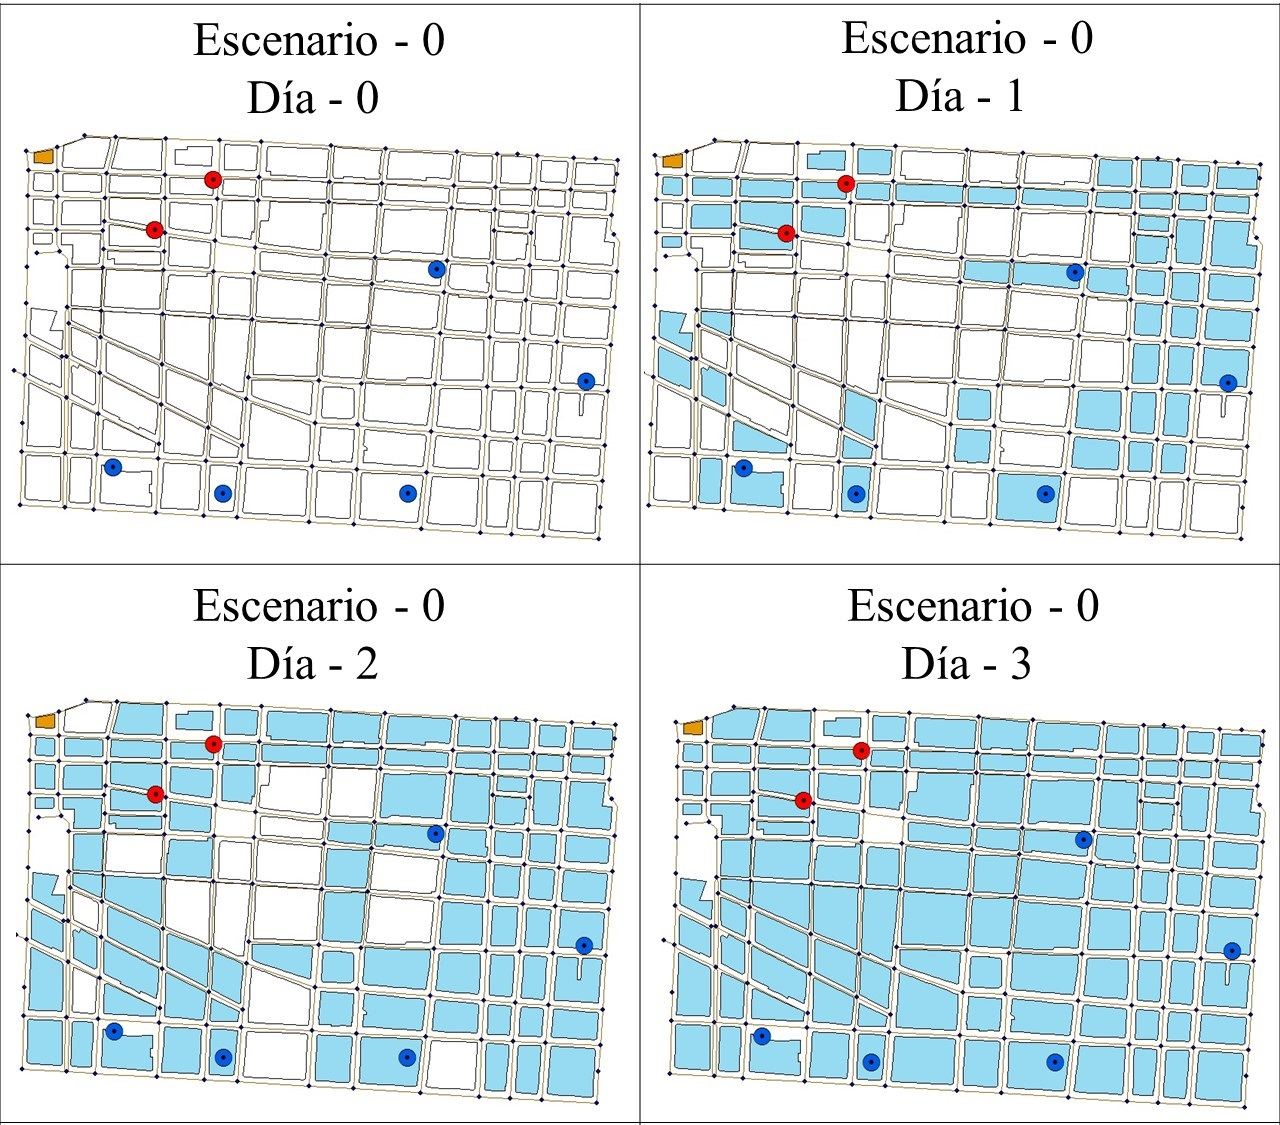
\includegraphics[scale=0.26]{Figuras/visu1.jpg} 
%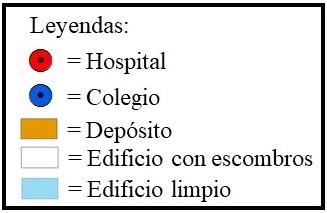
\includegraphics[scale=0.3]{Figuras/simb2.jpg}
%\caption{Escenario 0 - Visual; Fuente: Elaboración Propia}
%\label{visual0} 
%\end{figure}
%
%En cambio, en la figura \ref{visual1} se presenta la variación dentro de los primeros 3 días de trabajo, lo cual presenta un deficit en el escenario 1, a causa de la cantidad de edificios que contienen escobros a remover, en el día 3. se debe remarcar que es importante el factor de prioridad hacia los primeros días de trabajo, en caso de existir emergencias de utilización de inmobiliario. \\
%
%\begin{figure}[h!]
%\centering
%\includegraphics[scale=0.26]{Figuras/visu2.jpg} 
%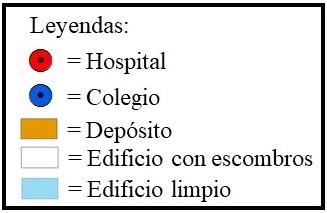
\includegraphics[scale=0.3]{Figuras/simb2.jpg}
%\caption{Escenario 0 - 1 - Visual; Fuente: Elaboración Propia}
%\label{visual1} 
%\end{figure}
%
%En la siguiente figura \ref{visual23}, se presenta la comparación entre el día 1 y día 2 de los escenarios 2 - 3, siendo comparado con el escenario base, quedando a la representado la velocidad en la limpieza de edificios, siendo el escenario 2 de menos recursos de camiones y más lento en cuanto a limpieza, y el escenario 3 el de mayor recursos de limpieza, y el más rapido de los 3 escenarios comparados.
%
%\begin{figure}[h!]
%\centering
%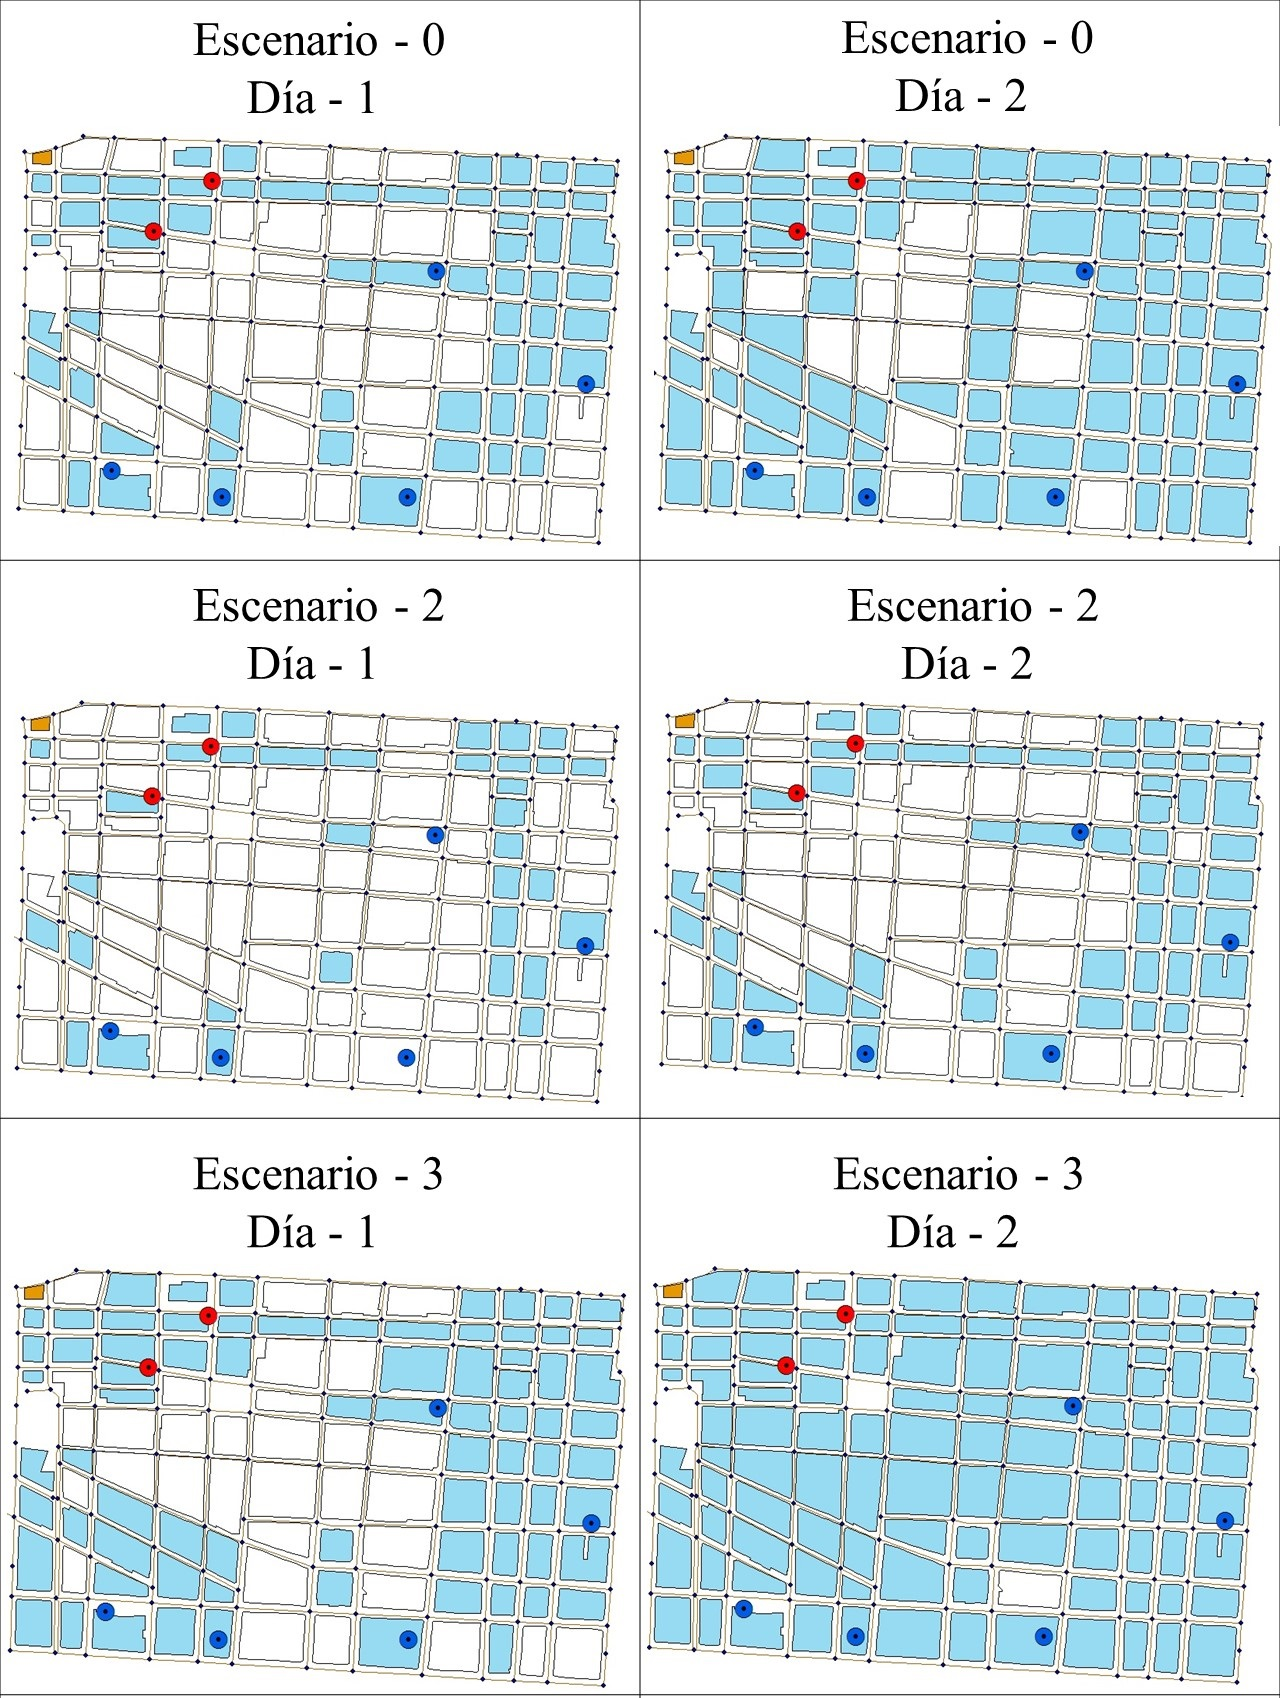
\includegraphics[scale=0.26]{Figuras/visu3.jpg} 
%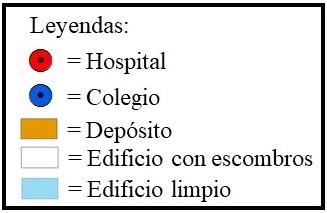
\includegraphics[scale=0.3]{Figuras/simb2.jpg}
%\caption{Escenario 2 - 3 - Visual; Fuente: Elaboración Propia}
%\label{visual23} 
%\end{figure}
%
%Finalmente en la figura \ref{visual456}, se presenta la comparación del escenario base con los escenarios con aumento de cantidad de volumento de escombros, comparando el día 1 con el día 3 de cada escenario. Obteniendo la conclusión que al aumentar la cantidad de escombros se ve afectado directamente la cantidad de edificios completamente limpios, dejando a la vista que el escenario con mejores resultados es el base, siendo el de menor volumen de escombros a remover.
%
%\begin{figure}[h!]
%\centering
%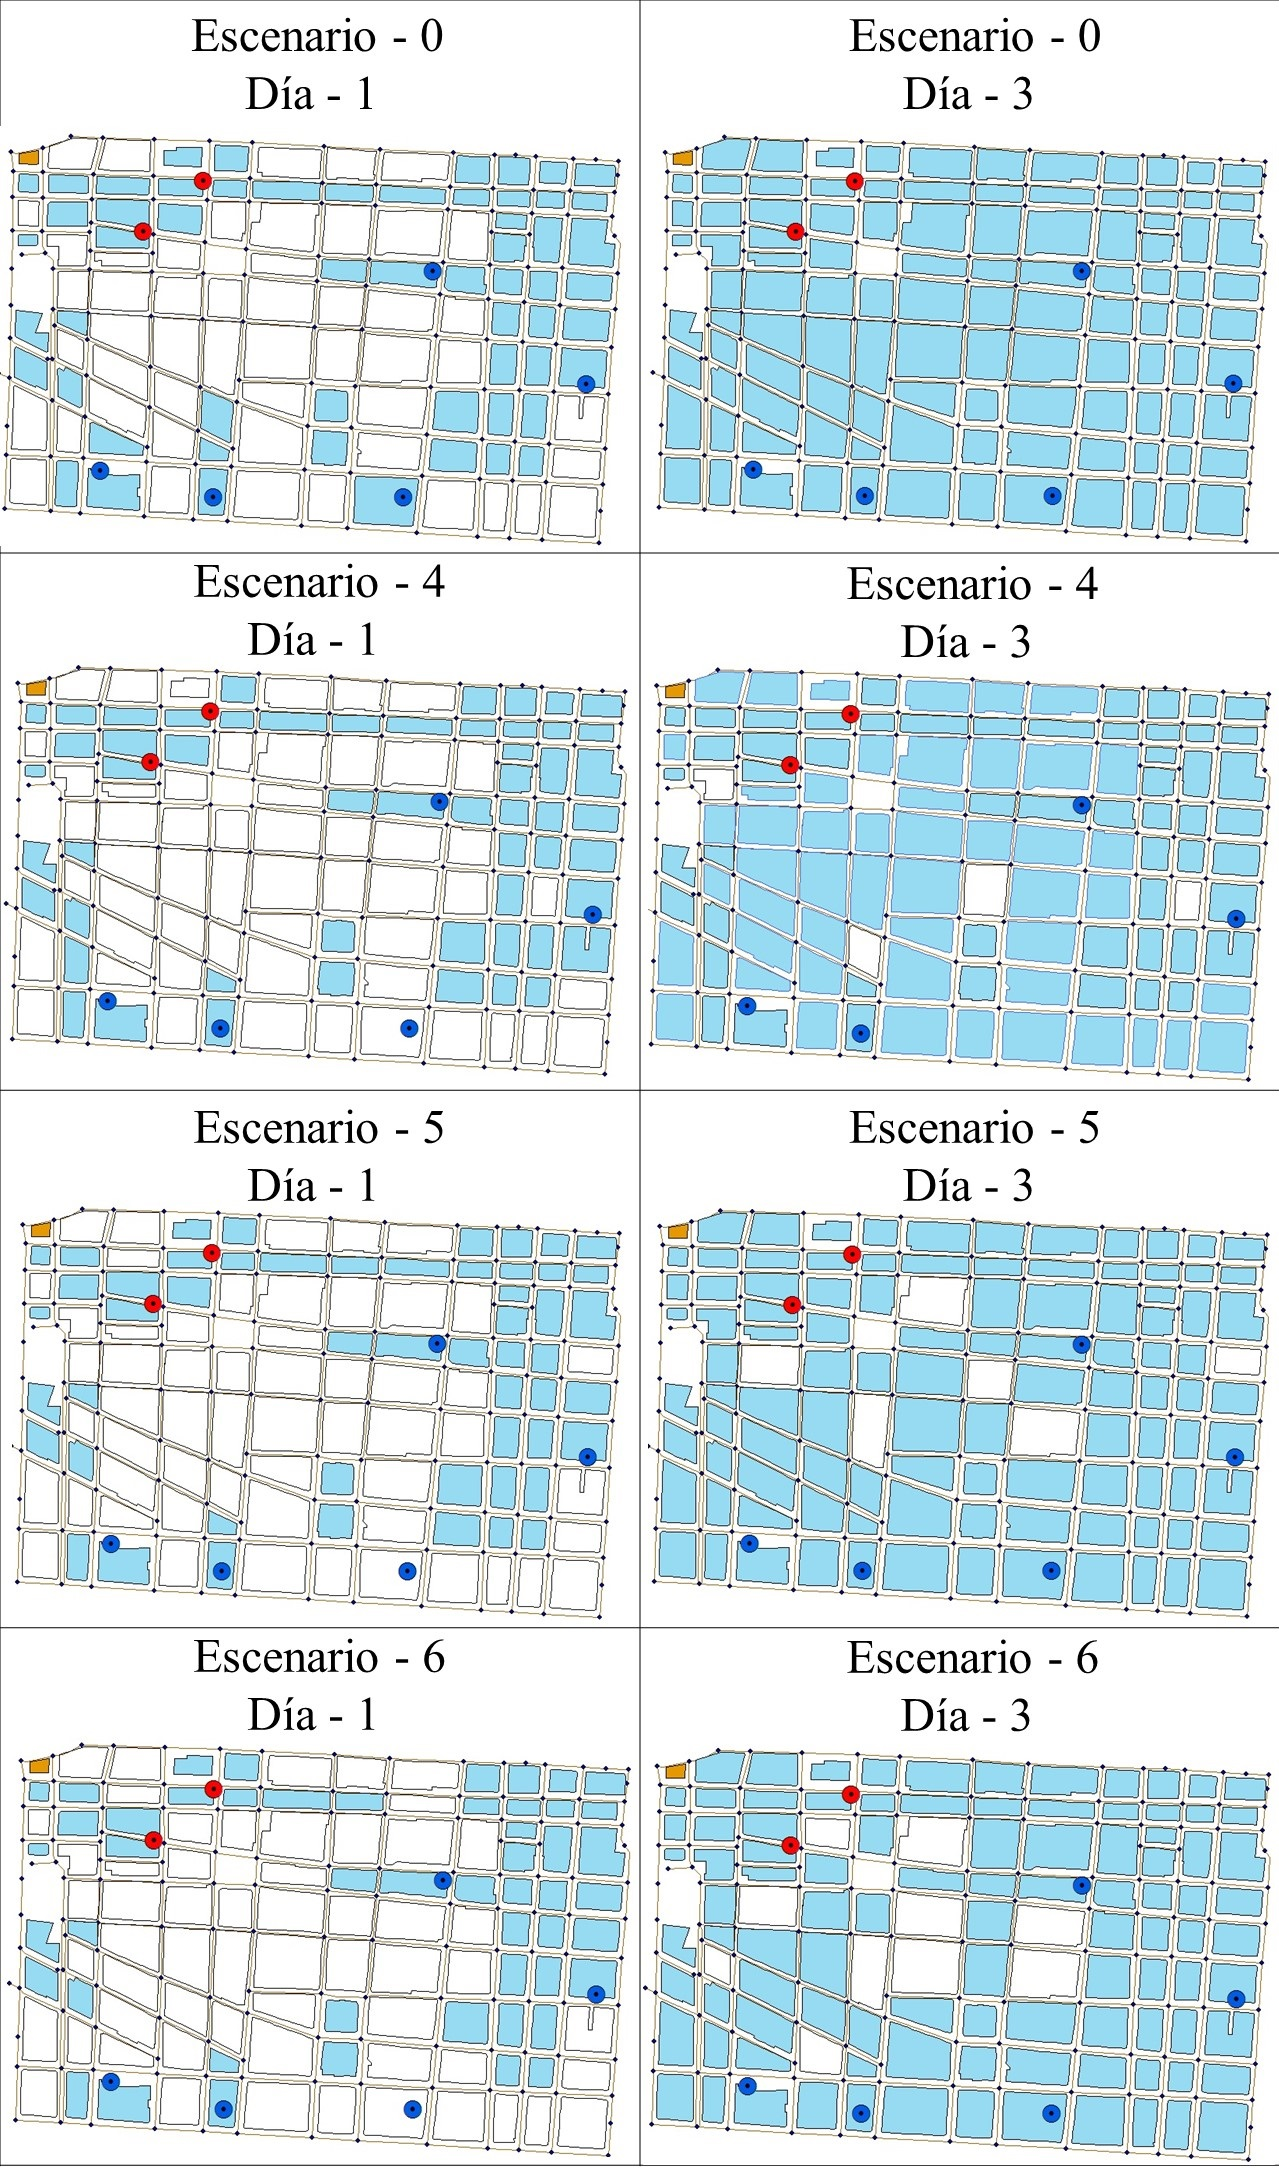
\includegraphics[scale=0.27]{Figuras/visu4.jpg} 
%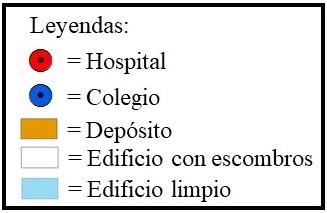
\includegraphics[scale=0.3]{Figuras/simb2.jpg}
%\caption{Escenario 4 - 5 - 6 - Visual; Fuente: Elaboración Propia}
%\label{visual456} 
%\end{figure}

%Los resultados son trabajados en este mismo instante. \citep{sismologia}

%%%%%%%%%%%%%%%%%%%%%%%%%%%%%       REFERENCIAS       %%%%%%%%%%%%%%%%%

\bibliographystyle{apalike}
\bibliography{references}

\end{document}